
% Default to the notebook output style

    


% Inherit from the specified cell style.




    
\documentclass[11pt]{article}

    
    
    \usepackage[T1]{fontenc}
    % Nicer default font (+ math font) than Computer Modern for most use cases
    \usepackage{mathpazo}

    % Basic figure setup, for now with no caption control since it's done
    % automatically by Pandoc (which extracts ![](path) syntax from Markdown).
    \usepackage{graphicx}
    % We will generate all images so they have a width \maxwidth. This means
    % that they will get their normal width if they fit onto the page, but
    % are scaled down if they would overflow the margins.
    \makeatletter
    \def\maxwidth{\ifdim\Gin@nat@width>\linewidth\linewidth
    \else\Gin@nat@width\fi}
    \makeatother
    \let\Oldincludegraphics\includegraphics
    % Set max figure width to be 80% of text width, for now hardcoded.
    \renewcommand{\includegraphics}[1]{\Oldincludegraphics[width=.8\maxwidth]{#1}}
    % Ensure that by default, figures have no caption (until we provide a
    % proper Figure object with a Caption API and a way to capture that
    % in the conversion process - todo).
    \usepackage{caption}
    \DeclareCaptionLabelFormat{nolabel}{}
    \captionsetup{labelformat=nolabel}

    \usepackage{adjustbox} % Used to constrain images to a maximum size 
    \usepackage{xcolor} % Allow colors to be defined
    \usepackage{enumerate} % Needed for markdown enumerations to work
    \usepackage{geometry} % Used to adjust the document margins
    \usepackage{amsmath} % Equations
    \usepackage{amssymb} % Equations
    \usepackage{textcomp} % defines textquotesingle
    % Hack from http://tex.stackexchange.com/a/47451/13684:
    \AtBeginDocument{%
        \def\PYZsq{\textquotesingle}% Upright quotes in Pygmentized code
    }
    \usepackage{upquote} % Upright quotes for verbatim code
    \usepackage{eurosym} % defines \euro
    \usepackage[mathletters]{ucs} % Extended unicode (utf-8) support
    \usepackage[utf8x]{inputenc} % Allow utf-8 characters in the tex document
    \usepackage{fancyvrb} % verbatim replacement that allows latex
    \usepackage{grffile} % extends the file name processing of package graphics 
                         % to support a larger range 
    % The hyperref package gives us a pdf with properly built
    % internal navigation ('pdf bookmarks' for the table of contents,
    % internal cross-reference links, web links for URLs, etc.)
    \usepackage{hyperref}
    \usepackage{longtable} % longtable support required by pandoc >1.10
    \usepackage{booktabs}  % table support for pandoc > 1.12.2
    \usepackage[inline]{enumitem} % IRkernel/repr support (it uses the enumerate* environment)
    \usepackage[normalem]{ulem} % ulem is needed to support strikethroughs (\sout)
                                % normalem makes italics be italics, not underlines
    

    
    
    % Colors for the hyperref package
    \definecolor{urlcolor}{rgb}{0,.145,.698}
    \definecolor{linkcolor}{rgb}{.71,0.21,0.01}
    \definecolor{citecolor}{rgb}{.12,.54,.11}

    % ANSI colors
    \definecolor{ansi-black}{HTML}{3E424D}
    \definecolor{ansi-black-intense}{HTML}{282C36}
    \definecolor{ansi-red}{HTML}{E75C58}
    \definecolor{ansi-red-intense}{HTML}{B22B31}
    \definecolor{ansi-green}{HTML}{00A250}
    \definecolor{ansi-green-intense}{HTML}{007427}
    \definecolor{ansi-yellow}{HTML}{DDB62B}
    \definecolor{ansi-yellow-intense}{HTML}{B27D12}
    \definecolor{ansi-blue}{HTML}{208FFB}
    \definecolor{ansi-blue-intense}{HTML}{0065CA}
    \definecolor{ansi-magenta}{HTML}{D160C4}
    \definecolor{ansi-magenta-intense}{HTML}{A03196}
    \definecolor{ansi-cyan}{HTML}{60C6C8}
    \definecolor{ansi-cyan-intense}{HTML}{258F8F}
    \definecolor{ansi-white}{HTML}{C5C1B4}
    \definecolor{ansi-white-intense}{HTML}{A1A6B2}

    % commands and environments needed by pandoc snippets
    % extracted from the output of `pandoc -s`
    \providecommand{\tightlist}{%
      \setlength{\itemsep}{0pt}\setlength{\parskip}{0pt}}
    \DefineVerbatimEnvironment{Highlighting}{Verbatim}{commandchars=\\\{\}}
    % Add ',fontsize=\small' for more characters per line
    \newenvironment{Shaded}{}{}
    \newcommand{\KeywordTok}[1]{\textcolor[rgb]{0.00,0.44,0.13}{\textbf{{#1}}}}
    \newcommand{\DataTypeTok}[1]{\textcolor[rgb]{0.56,0.13,0.00}{{#1}}}
    \newcommand{\DecValTok}[1]{\textcolor[rgb]{0.25,0.63,0.44}{{#1}}}
    \newcommand{\BaseNTok}[1]{\textcolor[rgb]{0.25,0.63,0.44}{{#1}}}
    \newcommand{\FloatTok}[1]{\textcolor[rgb]{0.25,0.63,0.44}{{#1}}}
    \newcommand{\CharTok}[1]{\textcolor[rgb]{0.25,0.44,0.63}{{#1}}}
    \newcommand{\StringTok}[1]{\textcolor[rgb]{0.25,0.44,0.63}{{#1}}}
    \newcommand{\CommentTok}[1]{\textcolor[rgb]{0.38,0.63,0.69}{\textit{{#1}}}}
    \newcommand{\OtherTok}[1]{\textcolor[rgb]{0.00,0.44,0.13}{{#1}}}
    \newcommand{\AlertTok}[1]{\textcolor[rgb]{1.00,0.00,0.00}{\textbf{{#1}}}}
    \newcommand{\FunctionTok}[1]{\textcolor[rgb]{0.02,0.16,0.49}{{#1}}}
    \newcommand{\RegionMarkerTok}[1]{{#1}}
    \newcommand{\ErrorTok}[1]{\textcolor[rgb]{1.00,0.00,0.00}{\textbf{{#1}}}}
    \newcommand{\NormalTok}[1]{{#1}}
    
    % Additional commands for more recent versions of Pandoc
    \newcommand{\ConstantTok}[1]{\textcolor[rgb]{0.53,0.00,0.00}{{#1}}}
    \newcommand{\SpecialCharTok}[1]{\textcolor[rgb]{0.25,0.44,0.63}{{#1}}}
    \newcommand{\VerbatimStringTok}[1]{\textcolor[rgb]{0.25,0.44,0.63}{{#1}}}
    \newcommand{\SpecialStringTok}[1]{\textcolor[rgb]{0.73,0.40,0.53}{{#1}}}
    \newcommand{\ImportTok}[1]{{#1}}
    \newcommand{\DocumentationTok}[1]{\textcolor[rgb]{0.73,0.13,0.13}{\textit{{#1}}}}
    \newcommand{\AnnotationTok}[1]{\textcolor[rgb]{0.38,0.63,0.69}{\textbf{\textit{{#1}}}}}
    \newcommand{\CommentVarTok}[1]{\textcolor[rgb]{0.38,0.63,0.69}{\textbf{\textit{{#1}}}}}
    \newcommand{\VariableTok}[1]{\textcolor[rgb]{0.10,0.09,0.49}{{#1}}}
    \newcommand{\ControlFlowTok}[1]{\textcolor[rgb]{0.00,0.44,0.13}{\textbf{{#1}}}}
    \newcommand{\OperatorTok}[1]{\textcolor[rgb]{0.40,0.40,0.40}{{#1}}}
    \newcommand{\BuiltInTok}[1]{{#1}}
    \newcommand{\ExtensionTok}[1]{{#1}}
    \newcommand{\PreprocessorTok}[1]{\textcolor[rgb]{0.74,0.48,0.00}{{#1}}}
    \newcommand{\AttributeTok}[1]{\textcolor[rgb]{0.49,0.56,0.16}{{#1}}}
    \newcommand{\InformationTok}[1]{\textcolor[rgb]{0.38,0.63,0.69}{\textbf{\textit{{#1}}}}}
    \newcommand{\WarningTok}[1]{\textcolor[rgb]{0.38,0.63,0.69}{\textbf{\textit{{#1}}}}}
    
    
    % Define a nice break command that doesn't care if a line doesn't already
    % exist.
    \def\br{\hspace*{\fill} \\* }
    % Math Jax compatability definitions
    \def\gt{>}
    \def\lt{<}
    % Document parameters
    \title{Assignment4 }
    
    
    

    % Pygments definitions
    
\makeatletter
\def\PY@reset{\let\PY@it=\relax \let\PY@bf=\relax%
    \let\PY@ul=\relax \let\PY@tc=\relax%
    \let\PY@bc=\relax \let\PY@ff=\relax}
\def\PY@tok#1{\csname PY@tok@#1\endcsname}
\def\PY@toks#1+{\ifx\relax#1\empty\else%
    \PY@tok{#1}\expandafter\PY@toks\fi}
\def\PY@do#1{\PY@bc{\PY@tc{\PY@ul{%
    \PY@it{\PY@bf{\PY@ff{#1}}}}}}}
\def\PY#1#2{\PY@reset\PY@toks#1+\relax+\PY@do{#2}}

\expandafter\def\csname PY@tok@w\endcsname{\def\PY@tc##1{\textcolor[rgb]{0.73,0.73,0.73}{##1}}}
\expandafter\def\csname PY@tok@c\endcsname{\let\PY@it=\textit\def\PY@tc##1{\textcolor[rgb]{0.25,0.50,0.50}{##1}}}
\expandafter\def\csname PY@tok@cp\endcsname{\def\PY@tc##1{\textcolor[rgb]{0.74,0.48,0.00}{##1}}}
\expandafter\def\csname PY@tok@k\endcsname{\let\PY@bf=\textbf\def\PY@tc##1{\textcolor[rgb]{0.00,0.50,0.00}{##1}}}
\expandafter\def\csname PY@tok@kp\endcsname{\def\PY@tc##1{\textcolor[rgb]{0.00,0.50,0.00}{##1}}}
\expandafter\def\csname PY@tok@kt\endcsname{\def\PY@tc##1{\textcolor[rgb]{0.69,0.00,0.25}{##1}}}
\expandafter\def\csname PY@tok@o\endcsname{\def\PY@tc##1{\textcolor[rgb]{0.40,0.40,0.40}{##1}}}
\expandafter\def\csname PY@tok@ow\endcsname{\let\PY@bf=\textbf\def\PY@tc##1{\textcolor[rgb]{0.67,0.13,1.00}{##1}}}
\expandafter\def\csname PY@tok@nb\endcsname{\def\PY@tc##1{\textcolor[rgb]{0.00,0.50,0.00}{##1}}}
\expandafter\def\csname PY@tok@nf\endcsname{\def\PY@tc##1{\textcolor[rgb]{0.00,0.00,1.00}{##1}}}
\expandafter\def\csname PY@tok@nc\endcsname{\let\PY@bf=\textbf\def\PY@tc##1{\textcolor[rgb]{0.00,0.00,1.00}{##1}}}
\expandafter\def\csname PY@tok@nn\endcsname{\let\PY@bf=\textbf\def\PY@tc##1{\textcolor[rgb]{0.00,0.00,1.00}{##1}}}
\expandafter\def\csname PY@tok@ne\endcsname{\let\PY@bf=\textbf\def\PY@tc##1{\textcolor[rgb]{0.82,0.25,0.23}{##1}}}
\expandafter\def\csname PY@tok@nv\endcsname{\def\PY@tc##1{\textcolor[rgb]{0.10,0.09,0.49}{##1}}}
\expandafter\def\csname PY@tok@no\endcsname{\def\PY@tc##1{\textcolor[rgb]{0.53,0.00,0.00}{##1}}}
\expandafter\def\csname PY@tok@nl\endcsname{\def\PY@tc##1{\textcolor[rgb]{0.63,0.63,0.00}{##1}}}
\expandafter\def\csname PY@tok@ni\endcsname{\let\PY@bf=\textbf\def\PY@tc##1{\textcolor[rgb]{0.60,0.60,0.60}{##1}}}
\expandafter\def\csname PY@tok@na\endcsname{\def\PY@tc##1{\textcolor[rgb]{0.49,0.56,0.16}{##1}}}
\expandafter\def\csname PY@tok@nt\endcsname{\let\PY@bf=\textbf\def\PY@tc##1{\textcolor[rgb]{0.00,0.50,0.00}{##1}}}
\expandafter\def\csname PY@tok@nd\endcsname{\def\PY@tc##1{\textcolor[rgb]{0.67,0.13,1.00}{##1}}}
\expandafter\def\csname PY@tok@s\endcsname{\def\PY@tc##1{\textcolor[rgb]{0.73,0.13,0.13}{##1}}}
\expandafter\def\csname PY@tok@sd\endcsname{\let\PY@it=\textit\def\PY@tc##1{\textcolor[rgb]{0.73,0.13,0.13}{##1}}}
\expandafter\def\csname PY@tok@si\endcsname{\let\PY@bf=\textbf\def\PY@tc##1{\textcolor[rgb]{0.73,0.40,0.53}{##1}}}
\expandafter\def\csname PY@tok@se\endcsname{\let\PY@bf=\textbf\def\PY@tc##1{\textcolor[rgb]{0.73,0.40,0.13}{##1}}}
\expandafter\def\csname PY@tok@sr\endcsname{\def\PY@tc##1{\textcolor[rgb]{0.73,0.40,0.53}{##1}}}
\expandafter\def\csname PY@tok@ss\endcsname{\def\PY@tc##1{\textcolor[rgb]{0.10,0.09,0.49}{##1}}}
\expandafter\def\csname PY@tok@sx\endcsname{\def\PY@tc##1{\textcolor[rgb]{0.00,0.50,0.00}{##1}}}
\expandafter\def\csname PY@tok@m\endcsname{\def\PY@tc##1{\textcolor[rgb]{0.40,0.40,0.40}{##1}}}
\expandafter\def\csname PY@tok@gh\endcsname{\let\PY@bf=\textbf\def\PY@tc##1{\textcolor[rgb]{0.00,0.00,0.50}{##1}}}
\expandafter\def\csname PY@tok@gu\endcsname{\let\PY@bf=\textbf\def\PY@tc##1{\textcolor[rgb]{0.50,0.00,0.50}{##1}}}
\expandafter\def\csname PY@tok@gd\endcsname{\def\PY@tc##1{\textcolor[rgb]{0.63,0.00,0.00}{##1}}}
\expandafter\def\csname PY@tok@gi\endcsname{\def\PY@tc##1{\textcolor[rgb]{0.00,0.63,0.00}{##1}}}
\expandafter\def\csname PY@tok@gr\endcsname{\def\PY@tc##1{\textcolor[rgb]{1.00,0.00,0.00}{##1}}}
\expandafter\def\csname PY@tok@ge\endcsname{\let\PY@it=\textit}
\expandafter\def\csname PY@tok@gs\endcsname{\let\PY@bf=\textbf}
\expandafter\def\csname PY@tok@gp\endcsname{\let\PY@bf=\textbf\def\PY@tc##1{\textcolor[rgb]{0.00,0.00,0.50}{##1}}}
\expandafter\def\csname PY@tok@go\endcsname{\def\PY@tc##1{\textcolor[rgb]{0.53,0.53,0.53}{##1}}}
\expandafter\def\csname PY@tok@gt\endcsname{\def\PY@tc##1{\textcolor[rgb]{0.00,0.27,0.87}{##1}}}
\expandafter\def\csname PY@tok@err\endcsname{\def\PY@bc##1{\setlength{\fboxsep}{0pt}\fcolorbox[rgb]{1.00,0.00,0.00}{1,1,1}{\strut ##1}}}
\expandafter\def\csname PY@tok@kc\endcsname{\let\PY@bf=\textbf\def\PY@tc##1{\textcolor[rgb]{0.00,0.50,0.00}{##1}}}
\expandafter\def\csname PY@tok@kd\endcsname{\let\PY@bf=\textbf\def\PY@tc##1{\textcolor[rgb]{0.00,0.50,0.00}{##1}}}
\expandafter\def\csname PY@tok@kn\endcsname{\let\PY@bf=\textbf\def\PY@tc##1{\textcolor[rgb]{0.00,0.50,0.00}{##1}}}
\expandafter\def\csname PY@tok@kr\endcsname{\let\PY@bf=\textbf\def\PY@tc##1{\textcolor[rgb]{0.00,0.50,0.00}{##1}}}
\expandafter\def\csname PY@tok@bp\endcsname{\def\PY@tc##1{\textcolor[rgb]{0.00,0.50,0.00}{##1}}}
\expandafter\def\csname PY@tok@fm\endcsname{\def\PY@tc##1{\textcolor[rgb]{0.00,0.00,1.00}{##1}}}
\expandafter\def\csname PY@tok@vc\endcsname{\def\PY@tc##1{\textcolor[rgb]{0.10,0.09,0.49}{##1}}}
\expandafter\def\csname PY@tok@vg\endcsname{\def\PY@tc##1{\textcolor[rgb]{0.10,0.09,0.49}{##1}}}
\expandafter\def\csname PY@tok@vi\endcsname{\def\PY@tc##1{\textcolor[rgb]{0.10,0.09,0.49}{##1}}}
\expandafter\def\csname PY@tok@vm\endcsname{\def\PY@tc##1{\textcolor[rgb]{0.10,0.09,0.49}{##1}}}
\expandafter\def\csname PY@tok@sa\endcsname{\def\PY@tc##1{\textcolor[rgb]{0.73,0.13,0.13}{##1}}}
\expandafter\def\csname PY@tok@sb\endcsname{\def\PY@tc##1{\textcolor[rgb]{0.73,0.13,0.13}{##1}}}
\expandafter\def\csname PY@tok@sc\endcsname{\def\PY@tc##1{\textcolor[rgb]{0.73,0.13,0.13}{##1}}}
\expandafter\def\csname PY@tok@dl\endcsname{\def\PY@tc##1{\textcolor[rgb]{0.73,0.13,0.13}{##1}}}
\expandafter\def\csname PY@tok@s2\endcsname{\def\PY@tc##1{\textcolor[rgb]{0.73,0.13,0.13}{##1}}}
\expandafter\def\csname PY@tok@sh\endcsname{\def\PY@tc##1{\textcolor[rgb]{0.73,0.13,0.13}{##1}}}
\expandafter\def\csname PY@tok@s1\endcsname{\def\PY@tc##1{\textcolor[rgb]{0.73,0.13,0.13}{##1}}}
\expandafter\def\csname PY@tok@mb\endcsname{\def\PY@tc##1{\textcolor[rgb]{0.40,0.40,0.40}{##1}}}
\expandafter\def\csname PY@tok@mf\endcsname{\def\PY@tc##1{\textcolor[rgb]{0.40,0.40,0.40}{##1}}}
\expandafter\def\csname PY@tok@mh\endcsname{\def\PY@tc##1{\textcolor[rgb]{0.40,0.40,0.40}{##1}}}
\expandafter\def\csname PY@tok@mi\endcsname{\def\PY@tc##1{\textcolor[rgb]{0.40,0.40,0.40}{##1}}}
\expandafter\def\csname PY@tok@il\endcsname{\def\PY@tc##1{\textcolor[rgb]{0.40,0.40,0.40}{##1}}}
\expandafter\def\csname PY@tok@mo\endcsname{\def\PY@tc##1{\textcolor[rgb]{0.40,0.40,0.40}{##1}}}
\expandafter\def\csname PY@tok@ch\endcsname{\let\PY@it=\textit\def\PY@tc##1{\textcolor[rgb]{0.25,0.50,0.50}{##1}}}
\expandafter\def\csname PY@tok@cm\endcsname{\let\PY@it=\textit\def\PY@tc##1{\textcolor[rgb]{0.25,0.50,0.50}{##1}}}
\expandafter\def\csname PY@tok@cpf\endcsname{\let\PY@it=\textit\def\PY@tc##1{\textcolor[rgb]{0.25,0.50,0.50}{##1}}}
\expandafter\def\csname PY@tok@c1\endcsname{\let\PY@it=\textit\def\PY@tc##1{\textcolor[rgb]{0.25,0.50,0.50}{##1}}}
\expandafter\def\csname PY@tok@cs\endcsname{\let\PY@it=\textit\def\PY@tc##1{\textcolor[rgb]{0.25,0.50,0.50}{##1}}}

\def\PYZbs{\char`\\}
\def\PYZus{\char`\_}
\def\PYZob{\char`\{}
\def\PYZcb{\char`\}}
\def\PYZca{\char`\^}
\def\PYZam{\char`\&}
\def\PYZlt{\char`\<}
\def\PYZgt{\char`\>}
\def\PYZsh{\char`\#}
\def\PYZpc{\char`\%}
\def\PYZdl{\char`\$}
\def\PYZhy{\char`\-}
\def\PYZsq{\char`\'}
\def\PYZdq{\char`\"}
\def\PYZti{\char`\~}
% for compatibility with earlier versions
\def\PYZat{@}
\def\PYZlb{[}
\def\PYZrb{]}
\makeatother


    % Exact colors from NB
    \definecolor{incolor}{rgb}{0.0, 0.0, 0.5}
    \definecolor{outcolor}{rgb}{0.545, 0.0, 0.0}



    
    % Prevent overflowing lines due to hard-to-break entities
    \sloppy 
    % Setup hyperref package
    \hypersetup{
      breaklinks=true,  % so long urls are correctly broken across lines
      colorlinks=true,
      urlcolor=urlcolor,
      linkcolor=linkcolor,
      citecolor=citecolor,
      }
    % Slightly bigger margins than the latex defaults
    
    \geometry{verbose,tmargin=1in,bmargin=1in,lmargin=1in,rmargin=1in}
    
    

    \begin{document}
    
    
    \maketitle
    
    

    
    \hypertarget{cse-252a-computer-vision-i-fall-2018---assignment-4}{%
\section{CSE 252A Computer Vision I Fall 2018 - Assignment
4}\label{cse-252a-computer-vision-i-fall-2018---assignment-4}}

\hypertarget{instructor-david-kriegman}{%
\subsubsection{Instructor: David
Kriegman}\label{instructor-david-kriegman}}

\hypertarget{assignment-published-on-wednesday-november-27-2018}{%
\subsubsection{Assignment Published On: Wednesday, November 27,
2018}\label{assignment-published-on-wednesday-november-27-2018}}

\hypertarget{due-on-friday-december-7-2018-1159-pm}{%
\subsubsection{Due On: Friday, December 7, 2018 11:59
pm}\label{due-on-friday-december-7-2018-1159-pm}}

\hypertarget{instructions}{%
\subsection{Instructions}\label{instructions}}

\begin{itemize}
\tightlist
\item
  Review the academic integrity and collaboration policies on the course
  website.
\item
  This assignment must be completed individually.
\item
  Programming aspects of this assignment must be completed using Python
  in this notebook.
\item
  If you want to modify the skeleton code, you can do so. This has been
  provided just to provide you with a framework for the solution.
\item
  You may use python packages for basic linear algebra (you can use
  numpy or scipy for basic operations), but you may not use packages
  that directly solve the problem.
\item
  If you are unsure about using a specific package or function, then ask
  the instructor and teaching assistants for clarification.
\item
  You must submit this notebook exported as a pdf. You must also submit
  this notebook as .ipynb file.
\item
  You must submit both files (.pdf and .ipynb) on Gradescope. You must
  mark each problem on Gradescope in the pdf.
\item
  \textbf{Late policy} - 10\% per day late penalty after due date up to
  3 days.
\end{itemize}

    \hypertarget{problem-1-optical-flow-10-pts}{%
\subsection{Problem 1: Optical Flow {[}10
pts{]}}\label{problem-1-optical-flow-10-pts}}

In this problem, the single scale Lucas-Kanade method for estimating
optical flow will be implemented, and the data needed for this problem
can be found in the folder `optical\_flow\_images'.

An example optical flow output is shown below - this is not a solution,
just an example output.
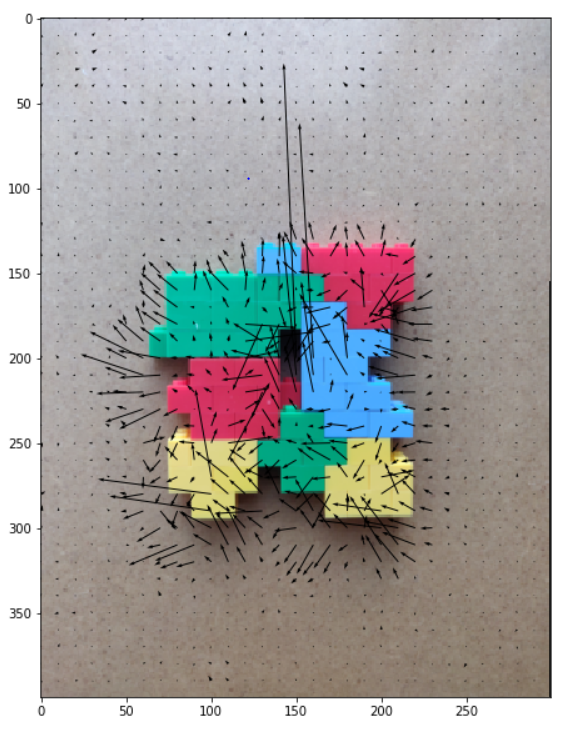
\includegraphics{optical_flow_images/sample_optical_flow_output.PNG}

    \hypertarget{part-1-lucas-kanade-implementation-5-pts}{%
\subsubsection{Part 1: Lucas-Kanade implementation {[}5
pts{]}}\label{part-1-lucas-kanade-implementation-5-pts}}

Implement the Lucas-Kanade method for estimating optical flow. The
function `LucasKanade' needs to be completed.

    \begin{Verbatim}[commandchars=\\\{\}]
{\color{incolor}In [{\color{incolor}76}]:} \PY{o}{\PYZpc{}}\PY{k}{matplotlib} inline 
         \PY{k+kn}{import} \PY{n+nn}{numpy} \PY{k}{as} \PY{n+nn}{np}
         \PY{k+kn}{import} \PY{n+nn}{matplotlib}\PY{n+nn}{.}\PY{n+nn}{pyplot} \PY{k}{as} \PY{n+nn}{plt}
         \PY{k+kn}{from} \PY{n+nn}{scipy}\PY{n+nn}{.}\PY{n+nn}{signal} \PY{k}{import} \PY{n}{convolve2d} \PY{k}{as} \PY{n}{conv2}
         
         \PY{k}{def} \PY{n+nf}{grayscale}\PY{p}{(}\PY{n}{img}\PY{p}{)}\PY{p}{:}
             \PY{l+s+sd}{\PYZsq{}\PYZsq{}\PYZsq{}}
         \PY{l+s+sd}{    Converts RGB image to Grayscale}
         \PY{l+s+sd}{    \PYZsq{}\PYZsq{}\PYZsq{}}
             \PY{n}{gray}\PY{o}{=}\PY{n}{np}\PY{o}{.}\PY{n}{zeros}\PY{p}{(}\PY{p}{(}\PY{n}{img}\PY{o}{.}\PY{n}{shape}\PY{p}{[}\PY{l+m+mi}{0}\PY{p}{]}\PY{p}{,}\PY{n}{img}\PY{o}{.}\PY{n}{shape}\PY{p}{[}\PY{l+m+mi}{1}\PY{p}{]}\PY{p}{)}\PY{p}{)}
             \PY{n}{gray}\PY{o}{=}\PY{n}{img}\PY{p}{[}\PY{p}{:}\PY{p}{,}\PY{p}{:}\PY{p}{,}\PY{l+m+mi}{0}\PY{p}{]}\PY{o}{*}\PY{l+m+mf}{0.2989}\PY{o}{+}\PY{n}{img}\PY{p}{[}\PY{p}{:}\PY{p}{,}\PY{p}{:}\PY{p}{,}\PY{l+m+mi}{1}\PY{p}{]}\PY{o}{*}\PY{l+m+mf}{0.5870}\PY{o}{+}\PY{n}{img}\PY{p}{[}\PY{p}{:}\PY{p}{,}\PY{p}{:}\PY{p}{,}\PY{l+m+mi}{2}\PY{p}{]}\PY{o}{*}\PY{l+m+mf}{0.1140}
             \PY{k}{return} \PY{n}{gray}
         
         \PY{k}{def} \PY{n+nf}{plot\PYZus{}optical\PYZus{}flow}\PY{p}{(}\PY{n}{img}\PY{p}{,}\PY{n}{U}\PY{p}{,}\PY{n}{V}\PY{p}{)}\PY{p}{:}
             \PY{l+s+sd}{\PYZsq{}\PYZsq{}\PYZsq{}}
         \PY{l+s+sd}{    Plots optical flow given U,V and one of the images}
         \PY{l+s+sd}{    \PYZsq{}\PYZsq{}\PYZsq{}}
             
             \PY{c+c1}{\PYZsh{} Change t if required, affects the number of arrows}
             \PY{c+c1}{\PYZsh{} t should be between 1 and min(U.shape[0],U.shape[1])}
             \PY{n}{t}\PY{o}{=}\PY{l+m+mi}{10} 
             
             \PY{c+c1}{\PYZsh{} Subsample U and V to get visually pleasing output}
             \PY{n}{U1} \PY{o}{=} \PY{n}{U}\PY{p}{[}\PY{p}{:}\PY{p}{:}\PY{n}{t}\PY{p}{,}\PY{p}{:}\PY{p}{:}\PY{n}{t}\PY{p}{]}
             \PY{n}{V1} \PY{o}{=} \PY{n}{V}\PY{p}{[}\PY{p}{:}\PY{p}{:}\PY{n}{t}\PY{p}{,}\PY{p}{:}\PY{p}{:}\PY{n}{t}\PY{p}{]}
             
             \PY{c+c1}{\PYZsh{} Create meshgrid of subsampled coordinates}
             \PY{n}{r}\PY{p}{,} \PY{n}{c} \PY{o}{=} \PY{n}{img}\PY{o}{.}\PY{n}{shape}\PY{p}{[}\PY{l+m+mi}{0}\PY{p}{]}\PY{p}{,}\PY{n}{img}\PY{o}{.}\PY{n}{shape}\PY{p}{[}\PY{l+m+mi}{1}\PY{p}{]}
             \PY{n}{cols}\PY{p}{,}\PY{n}{rows} \PY{o}{=} \PY{n}{np}\PY{o}{.}\PY{n}{meshgrid}\PY{p}{(}\PY{n}{np}\PY{o}{.}\PY{n}{linspace}\PY{p}{(}\PY{l+m+mi}{0}\PY{p}{,}\PY{n}{c}\PY{o}{\PYZhy{}}\PY{l+m+mi}{1}\PY{p}{,}\PY{n}{c}\PY{p}{)}\PY{p}{,} \PY{n}{np}\PY{o}{.}\PY{n}{linspace}\PY{p}{(}\PY{l+m+mi}{0}\PY{p}{,}\PY{n}{r}\PY{o}{\PYZhy{}}\PY{l+m+mi}{1}\PY{p}{,}\PY{n}{r}\PY{p}{)}\PY{p}{)}
             \PY{n}{cols} \PY{o}{=} \PY{n}{cols}\PY{p}{[}\PY{p}{:}\PY{p}{:}\PY{n}{t}\PY{p}{,}\PY{p}{:}\PY{p}{:}\PY{n}{t}\PY{p}{]}
             \PY{n}{rows} \PY{o}{=} \PY{n}{rows}\PY{p}{[}\PY{p}{:}\PY{p}{:}\PY{n}{t}\PY{p}{,}\PY{p}{:}\PY{p}{:}\PY{n}{t}\PY{p}{]}
             
             \PY{c+c1}{\PYZsh{} Plot optical flow}
             \PY{n}{plt}\PY{o}{.}\PY{n}{figure}\PY{p}{(}\PY{n}{figsize}\PY{o}{=}\PY{p}{(}\PY{l+m+mi}{10}\PY{p}{,}\PY{l+m+mi}{10}\PY{p}{)}\PY{p}{)}
             \PY{n}{plt}\PY{o}{.}\PY{n}{imshow}\PY{p}{(}\PY{n}{img}\PY{p}{)}
             \PY{n}{plt}\PY{o}{.}\PY{n}{quiver}\PY{p}{(}\PY{n}{cols}\PY{p}{,}\PY{n}{rows}\PY{p}{,}\PY{n}{U1}\PY{p}{,}\PY{n}{V1}\PY{p}{)}
             \PY{n}{plt}\PY{o}{.}\PY{n}{show}\PY{p}{(}\PY{p}{)}
         
         \PY{n}{images}\PY{o}{=}\PY{p}{[}\PY{p}{]}
         \PY{k}{for} \PY{n}{i} \PY{o+ow}{in} \PY{n+nb}{range}\PY{p}{(}\PY{l+m+mi}{1}\PY{p}{,}\PY{l+m+mi}{5}\PY{p}{)}\PY{p}{:}
             \PY{n}{images}\PY{o}{.}\PY{n}{append}\PY{p}{(}\PY{n}{plt}\PY{o}{.}\PY{n}{imread}\PY{p}{(}\PY{l+s+s1}{\PYZsq{}}\PY{l+s+s1}{optical\PYZus{}flow\PYZus{}images/im}\PY{l+s+s1}{\PYZsq{}}\PY{o}{+}\PY{n+nb}{str}\PY{p}{(}\PY{n}{i}\PY{p}{)}\PY{o}{+}\PY{l+s+s1}{\PYZsq{}}\PY{l+s+s1}{.png}\PY{l+s+s1}{\PYZsq{}}\PY{p}{)}\PY{p}{)}
\end{Verbatim}


    \begin{Verbatim}[commandchars=\\\{\}]
{\color{incolor}In [{\color{incolor}77}]:} \PY{k}{def} \PY{n+nf}{imconv}\PY{p}{(}\PY{n}{img}\PY{p}{,} \PY{n}{operator}\PY{p}{)}\PY{p}{:}
             \PY{n}{conved\PYZus{}img} \PY{o}{=} \PY{n}{np}\PY{o}{.}\PY{n}{zeros}\PY{p}{(}\PY{n}{img}\PY{o}{.}\PY{n}{shape}\PY{p}{)}  
             \PY{n}{r\PYZus{}center} \PY{o}{=} \PY{n+nb}{int}\PY{p}{(}\PY{p}{(}\PY{n}{operator}\PY{o}{.}\PY{n}{shape}\PY{p}{[}\PY{l+m+mi}{0}\PY{p}{]}\PY{o}{\PYZhy{}}\PY{l+m+mi}{1}\PY{p}{)}\PY{o}{/}\PY{l+m+mi}{2}\PY{p}{)}
             \PY{n}{c\PYZus{}center} \PY{o}{=} \PY{n+nb}{int}\PY{p}{(}\PY{p}{(}\PY{n}{operator}\PY{o}{.}\PY{n}{shape}\PY{p}{[}\PY{l+m+mi}{1}\PY{p}{]}\PY{o}{\PYZhy{}}\PY{l+m+mi}{1}\PY{p}{)}\PY{o}{/}\PY{l+m+mi}{2}\PY{p}{)}
             \PY{n}{num\PYZus{}row}\PY{p}{,} \PY{n}{num\PYZus{}col} \PY{o}{=} \PY{n}{img}\PY{o}{.}\PY{n}{shape}
         
             \PY{k}{for} \PY{n}{i} \PY{o+ow}{in} \PY{n+nb}{range}\PY{p}{(}\PY{n}{r\PYZus{}center}\PY{p}{,} \PY{n}{num\PYZus{}row}\PY{o}{\PYZhy{}}\PY{n}{r\PYZus{}center}\PY{p}{)}\PY{p}{:}
                 \PY{k}{for} \PY{n}{j} \PY{o+ow}{in} \PY{n+nb}{range}\PY{p}{(}\PY{n}{c\PYZus{}center}\PY{p}{,} \PY{n}{num\PYZus{}col}\PY{o}{\PYZhy{}}\PY{n}{c\PYZus{}center}\PY{p}{)}\PY{p}{:}
                     \PY{n}{conved\PYZus{}img}\PY{p}{[}\PY{n}{i}\PY{p}{]}\PY{p}{[}\PY{n}{j}\PY{p}{]} \PY{o}{=} \PY{p}{(}\PY{n}{img}\PY{p}{[}\PY{p}{(}\PY{n}{i}\PY{o}{\PYZhy{}}\PY{n}{r\PYZus{}center}\PY{p}{)}\PY{p}{:}\PY{p}{(}\PY{n}{i}\PY{o}{+}\PY{n}{r\PYZus{}center}\PY{o}{+}\PY{l+m+mi}{1}\PY{p}{)}\PY{p}{,}\PYZbs{}
                                             \PY{p}{(}\PY{n}{j}\PY{o}{\PYZhy{}}\PY{n}{c\PYZus{}center}\PY{p}{)}\PY{p}{:}\PY{p}{(}\PY{n}{j}\PY{o}{+}\PY{n}{c\PYZus{}center}\PY{o}{+}\PY{l+m+mi}{1}\PY{p}{)}\PY{p}{]} \PY{o}{*} \PY{n}{operator}\PY{p}{)}\PY{o}{.}\PY{n}{sum}\PY{p}{(}\PY{p}{)}
             \PY{k}{return} \PY{n}{conved\PYZus{}img} \PY{c+c1}{\PYZsh{}[r\PYZus{}center : (num\PYZus{}row\PYZhy{}r\PYZus{}center), c\PYZus{}center : (num\PYZus{}col\PYZhy{}c\PYZus{}center)]}
         
         
         
         
         
         \PY{k}{def} \PY{n+nf}{LucasKanade}\PY{p}{(}\PY{n}{im1}\PY{p}{,} \PY{n}{im2}\PY{p}{,} \PY{n}{windowSize}\PY{p}{)}\PY{p}{:}
             \PY{l+s+sd}{\PYZsq{}\PYZsq{}\PYZsq{}}
         \PY{l+s+sd}{    Inputs: the two images and window size}
         \PY{l+s+sd}{    Return U,V}
         \PY{l+s+sd}{    \PYZsq{}\PYZsq{}\PYZsq{}}
             \PY{n}{U} \PY{o}{=} \PY{n}{np}\PY{o}{.}\PY{n}{zeros}\PY{p}{(}\PY{n}{im1}\PY{o}{.}\PY{n}{shape}\PY{p}{)}
             \PY{n}{V} \PY{o}{=} \PY{n}{np}\PY{o}{.}\PY{n}{zeros}\PY{p}{(}\PY{n}{im1}\PY{o}{.}\PY{n}{shape}\PY{p}{)}
             
             \PY{l+s+sd}{\PYZsq{}\PYZsq{}\PYZsq{}}
         \PY{l+s+sd}{    Your code here}
         \PY{l+s+sd}{    \PYZsq{}\PYZsq{}\PYZsq{}}
             \PY{n}{sum\PYZus{}window} \PY{o}{=} \PY{n}{np}\PY{o}{.}\PY{n}{ones}\PY{p}{(}\PY{p}{(}\PY{n}{windowSize}\PY{p}{,} \PY{n}{windowSize}\PY{p}{)}\PY{p}{)}
             
             \PY{n}{img\PYZus{}dy}\PY{p}{,} \PY{n}{img\PYZus{}dx} \PY{o}{=} \PY{n}{np}\PY{o}{.}\PY{n}{gradient}\PY{p}{(}\PY{n}{im1}\PY{p}{)} \PY{c+c1}{\PYZsh{} y is row, x i column}
             \PY{n}{img\PYZus{}di} \PY{o}{=} \PY{n}{im2} \PY{o}{\PYZhy{}} \PY{n}{im1}
             
             \PY{n}{img\PYZus{}dxdx} \PY{o}{=} \PY{n}{img\PYZus{}dx} \PY{o}{*} \PY{n}{img\PYZus{}dx}
             \PY{n}{img\PYZus{}dydy} \PY{o}{=} \PY{n}{img\PYZus{}dy} \PY{o}{*} \PY{n}{img\PYZus{}dy}
             \PY{n}{img\PYZus{}dxdy} \PY{o}{=} \PY{n}{img\PYZus{}dx} \PY{o}{*} \PY{n}{img\PYZus{}dy}
             \PY{n}{img\PYZus{}dxdi} \PY{o}{=} \PY{n}{img\PYZus{}dx} \PY{o}{*} \PY{n}{img\PYZus{}di}
             \PY{n}{img\PYZus{}dydi} \PY{o}{=} \PY{n}{img\PYZus{}dy} \PY{o}{*} \PY{n}{img\PYZus{}di}
             
             
             \PY{n}{cov\PYZus{}sum\PYZus{}dxdx} \PY{o}{=} \PY{n}{imconv}\PY{p}{(}\PY{n}{img\PYZus{}dxdx}\PY{p}{,} \PY{n}{sum\PYZus{}window}\PY{p}{)}
             \PY{n}{cov\PYZus{}sum\PYZus{}dxdy} \PY{o}{=} \PY{n}{imconv}\PY{p}{(}\PY{n}{img\PYZus{}dxdy}\PY{p}{,} \PY{n}{sum\PYZus{}window}\PY{p}{)}
             \PY{n}{cov\PYZus{}sum\PYZus{}dydy} \PY{o}{=} \PY{n}{imconv}\PY{p}{(}\PY{n}{img\PYZus{}dydy}\PY{p}{,} \PY{n}{sum\PYZus{}window}\PY{p}{)}
             
             \PY{n}{cov\PYZus{}sum\PYZus{}dxdi} \PY{o}{=} \PY{n}{imconv}\PY{p}{(}\PY{n}{img\PYZus{}dxdi}\PY{p}{,} \PY{n}{sum\PYZus{}window}\PY{p}{)}
             \PY{n}{cov\PYZus{}sum\PYZus{}dydi} \PY{o}{=} \PY{n}{imconv}\PY{p}{(}\PY{n}{img\PYZus{}dydi}\PY{p}{,} \PY{n}{sum\PYZus{}window}\PY{p}{)}
             
             
             \PY{k}{for} \PY{n}{i} \PY{o+ow}{in} \PY{n+nb}{range}\PY{p}{(}\PY{n}{im1}\PY{o}{.}\PY{n}{shape}\PY{p}{[}\PY{l+m+mi}{0}\PY{p}{]}\PY{p}{)}\PY{p}{:}
                 \PY{k}{for} \PY{n}{j} \PY{o+ow}{in} \PY{n+nb}{range}\PY{p}{(}\PY{n}{im1}\PY{o}{.}\PY{n}{shape}\PY{p}{[}\PY{l+m+mi}{1}\PY{p}{]}\PY{p}{)}\PY{p}{:}
                     \PY{n}{M} \PY{o}{=} \PY{n}{np}\PY{o}{.}\PY{n}{array}\PY{p}{(}\PY{p}{[}\PY{p}{[}\PY{n}{cov\PYZus{}sum\PYZus{}dxdx}\PY{p}{[}\PY{n}{i}\PY{p}{]}\PY{p}{[}\PY{n}{j}\PY{p}{]}\PY{p}{,} \PY{n}{cov\PYZus{}sum\PYZus{}dxdy}\PY{p}{[}\PY{n}{i}\PY{p}{]}\PY{p}{[}\PY{n}{j}\PY{p}{]}\PY{p}{]}\PY{p}{,} 
                                   \PY{p}{[}\PY{n}{cov\PYZus{}sum\PYZus{}dxdy}\PY{p}{[}\PY{n}{i}\PY{p}{]}\PY{p}{[}\PY{n}{j}\PY{p}{]}\PY{p}{,} \PY{n}{cov\PYZus{}sum\PYZus{}dydy}\PY{p}{[}\PY{n}{i}\PY{p}{]}\PY{p}{[}\PY{n}{j}\PY{p}{]}\PY{p}{]}\PY{p}{]}\PY{p}{)}
                     
                     \PY{n}{b} \PY{o}{=} \PY{o}{\PYZhy{}} \PY{n}{np}\PY{o}{.}\PY{n}{array}\PY{p}{(}\PY{p}{[}\PY{p}{[}\PY{n}{cov\PYZus{}sum\PYZus{}dxdi}\PY{p}{[}\PY{n}{i}\PY{p}{]}\PY{p}{[}\PY{n}{j}\PY{p}{]}\PY{p}{]}\PY{p}{,} \PY{p}{[}\PY{n}{cov\PYZus{}sum\PYZus{}dydi}\PY{p}{[}\PY{n}{i}\PY{p}{]}\PY{p}{[}\PY{n}{j}\PY{p}{]}\PY{p}{]}\PY{p}{]}\PY{p}{)}
                     
                     \PY{n}{result} \PY{o}{=} \PY{n}{np}\PY{o}{.}\PY{n}{linalg}\PY{o}{.}\PY{n}{pinv}\PY{p}{(}\PY{n}{M}\PY{p}{)}\PY{o}{.}\PY{n}{dot}\PY{p}{(}\PY{n}{b}\PY{p}{)}
                     \PY{n}{U}\PY{p}{[}\PY{n}{i}\PY{p}{]}\PY{p}{[}\PY{n}{j}\PY{p}{]} \PY{o}{=} \PY{n}{result}\PY{p}{[}\PY{l+m+mi}{0}\PY{p}{]}\PY{p}{[}\PY{l+m+mi}{0}\PY{p}{]}
                     \PY{n}{V}\PY{p}{[}\PY{n}{i}\PY{p}{]}\PY{p}{[}\PY{n}{j}\PY{p}{]} \PY{o}{=} \PY{n}{result}\PY{p}{[}\PY{l+m+mi}{1}\PY{p}{]}\PY{p}{[}\PY{l+m+mi}{0}\PY{p}{]}
                     
             \PY{k}{return} \PY{n}{U}\PY{p}{,}\PY{n}{V}
\end{Verbatim}


    \hypertarget{part-2-window-size-2-pts}{%
\subsubsection{Part 2: Window size {[}2
pts{]}}\label{part-2-window-size-2-pts}}

Plot optical flow for the pair of images im1 and im2 for at least 3
different window sizes which leads to observable difference in the
results. Comment on the effect of window size on results and justify.

    \begin{Verbatim}[commandchars=\\\{\}]
{\color{incolor}In [{\color{incolor}11}]:} \PY{c+c1}{\PYZsh{} Example code, change as required}
         \PY{n}{window}\PY{o}{=}\PY{l+m+mi}{5}
         
         \PY{k}{for} \PY{n}{window} \PY{o+ow}{in} \PY{p}{[}\PY{l+m+mi}{5}\PY{p}{,} \PY{l+m+mi}{11}\PY{p}{,} \PY{l+m+mi}{15}\PY{p}{]}\PY{p}{:}
             \PY{n}{U}\PY{p}{,} \PY{n}{V}\PY{o}{=}\PY{n}{LucasKanade}\PY{p}{(}\PY{n}{grayscale}\PY{p}{(}\PY{n}{images}\PY{p}{[}\PY{l+m+mi}{0}\PY{p}{]}\PY{p}{)}\PY{p}{,}\PY{n}{grayscale}\PY{p}{(}\PY{n}{images}\PY{p}{[}\PY{l+m+mi}{1}\PY{p}{]}\PY{p}{)}\PY{p}{,}\PY{n}{window}\PY{p}{)}
             \PY{n}{plot\PYZus{}optical\PYZus{}flow}\PY{p}{(}\PY{n}{images}\PY{p}{[}\PY{l+m+mi}{0}\PY{p}{]}\PY{p}{,}\PY{n}{U}\PY{p}{,}\PY{n}{V}\PY{p}{)}
\end{Verbatim}


    \begin{center}
    \adjustimage{max size={0.9\linewidth}{0.9\paperheight}}{output_6_0.png}
    \end{center}
    { \hspace*{\fill} \\}
    
    \begin{center}
    \adjustimage{max size={0.9\linewidth}{0.9\paperheight}}{output_6_1.png}
    \end{center}
    { \hspace*{\fill} \\}
    
    \begin{center}
    \adjustimage{max size={0.9\linewidth}{0.9\paperheight}}{output_6_2.png}
    \end{center}
    { \hspace*{\fill} \\}
    
    In general, with appropriate large window size, the optical flow result
looks more accurate then results from smaller window size.

    \hypertarget{part-3-all-pairs-3-pts}{%
\subsubsection{Part 3: All pairs {[}3
pts{]}}\label{part-3-all-pairs-3-pts}}

Find optical flow for the pairs (im1,im2), (im1,im3), (im1,im4) using a
good window size. Does the optical flow result seem consistent with
visual inspection? Comment on the type of motion indicated by results
and visual inspection and explain why they might be consistent or
inconsistent.

    \begin{Verbatim}[commandchars=\\\{\}]
{\color{incolor}In [{\color{incolor}96}]:} \PY{c+c1}{\PYZsh{} Example code, change as required}
         \PY{n}{window} \PY{o}{=} \PY{l+m+mi}{21}
         
         \PY{n+nb}{print}\PY{p}{(}\PY{l+s+s1}{\PYZsq{}}\PY{l+s+s1}{im1 and im2}\PY{l+s+s1}{\PYZsq{}}\PY{p}{)}
         \PY{n}{U}\PY{p}{,} \PY{n}{V}\PY{o}{=}\PY{n}{LucasKanade}\PY{p}{(}\PY{n}{grayscale}\PY{p}{(}\PY{n}{images}\PY{p}{[}\PY{l+m+mi}{0}\PY{p}{]}\PY{p}{)}\PY{p}{,}\PY{n}{grayscale}\PY{p}{(}\PY{n}{images}\PY{p}{[}\PY{l+m+mi}{1}\PY{p}{]}\PY{p}{)}\PY{p}{,}\PY{n}{window}\PY{p}{)}
         \PY{n}{plot\PYZus{}optical\PYZus{}flow}\PY{p}{(}\PY{n}{images}\PY{p}{[}\PY{l+m+mi}{0}\PY{p}{]}\PY{p}{,}\PY{n}{U}\PY{p}{,}\PY{n}{V}\PY{p}{)}
         
         \PY{n+nb}{print}\PY{p}{(}\PY{l+s+s1}{\PYZsq{}}\PY{l+s+s1}{im1 and im3}\PY{l+s+s1}{\PYZsq{}}\PY{p}{)}
         \PY{n}{U}\PY{p}{,} \PY{n}{V}\PY{o}{=}\PY{n}{LucasKanade}\PY{p}{(}\PY{n}{grayscale}\PY{p}{(}\PY{n}{images}\PY{p}{[}\PY{l+m+mi}{0}\PY{p}{]}\PY{p}{)}\PY{p}{,}\PY{n}{grayscale}\PY{p}{(}\PY{n}{images}\PY{p}{[}\PY{l+m+mi}{2}\PY{p}{]}\PY{p}{)}\PY{p}{,}\PY{n}{window}\PY{p}{)}
         \PY{n}{plot\PYZus{}optical\PYZus{}flow}\PY{p}{(}\PY{n}{images}\PY{p}{[}\PY{l+m+mi}{0}\PY{p}{]}\PY{p}{,}\PY{n}{U}\PY{p}{,}\PY{n}{V}\PY{p}{)}
         
         \PY{n+nb}{print}\PY{p}{(}\PY{l+s+s1}{\PYZsq{}}\PY{l+s+s1}{im1 and im4}\PY{l+s+s1}{\PYZsq{}}\PY{p}{)}
         \PY{n}{U}\PY{p}{,} \PY{n}{V}\PY{o}{=}\PY{n}{LucasKanade}\PY{p}{(}\PY{n}{grayscale}\PY{p}{(}\PY{n}{images}\PY{p}{[}\PY{l+m+mi}{0}\PY{p}{]}\PY{p}{)}\PY{p}{,}\PY{n}{grayscale}\PY{p}{(}\PY{n}{images}\PY{p}{[}\PY{l+m+mi}{3}\PY{p}{]}\PY{p}{)}\PY{p}{,}\PY{n}{window}\PY{p}{)}
         \PY{n}{plot\PYZus{}optical\PYZus{}flow}\PY{p}{(}\PY{n}{images}\PY{p}{[}\PY{l+m+mi}{0}\PY{p}{]}\PY{p}{,}\PY{n}{U}\PY{p}{,}\PY{n}{V}\PY{p}{)}
\end{Verbatim}


    \begin{Verbatim}[commandchars=\\\{\}]
im1 and im2

    \end{Verbatim}

    \begin{center}
    \adjustimage{max size={0.9\linewidth}{0.9\paperheight}}{output_9_1.png}
    \end{center}
    { \hspace*{\fill} \\}
    
    \begin{Verbatim}[commandchars=\\\{\}]
im1 and im3

    \end{Verbatim}

    \begin{center}
    \adjustimage{max size={0.9\linewidth}{0.9\paperheight}}{output_9_3.png}
    \end{center}
    { \hspace*{\fill} \\}
    
    \begin{Verbatim}[commandchars=\\\{\}]
im1 and im4

    \end{Verbatim}

    \begin{center}
    \adjustimage{max size={0.9\linewidth}{0.9\paperheight}}{output_9_5.png}
    \end{center}
    { \hspace*{\fill} \\}
    
    For im1 to im2, the ground truth is moving left, and in this optical
flow result most arrows are consistent moving left. For im1 to im3, the
ground truth is rotating clockwise, and in this optical flow result most
arrows are consistent clockwise rotating. For im1 to im4, the groudn
truth operation is zoom, and in optical flow result most arrow are
pointing to outside.

In general, most optical flow arrows are consistent to its inspection,
but some are not. It may be the algorithm is based on brightness
constancy and motion of brightness patterns, and some pixel may not
perfect obey this rule. Also, the calculation about this flow too much
depend on its window size, and is easily contaminated by its surrounding
pixels.

    \hypertarget{problem-2-machine-learning-12-pts}{%
\subsection{Problem 2: Machine Learning {[}12
pts{]}}\label{problem-2-machine-learning-12-pts}}

In this problem, you will implement several machine learning solutions
for computer vision problems.

    \hypertarget{part-1-initial-setup-1-pts}{%
\subsubsection{Part 1: Initial setup {[}1
pts{]}}\label{part-1-initial-setup-1-pts}}

Follow the directions on https://www.tensorflow.org/install/ to install
Tensorflow on your computer. If you are using the Anaconda distribution
for python, you can check out
https://www.anaconda.com/blog/developer-blog/tensorflow-in-anaconda/.

Note: You will not need GPU support for this assignment so don't worry
if you don't have one. Furthermore, installing with GPU support is often
more difficult to configure so it is suggested that you install the CPU
only version.

Run the tensorflow hello world snippet below to verify your instalation.

Download the MNIST data from http://yann.lecun.com/exdb/mnist/.

Download the 4 zipped files, extract them into one folder, and change
the variable `path' in the code below. (Code taken from
https://gist.github.com/akesling/5358964 )

Plot one random example image corresponding to each label from training
data.

    \begin{Verbatim}[commandchars=\\\{\}]
{\color{incolor}In [{\color{incolor}78}]:} \PY{k+kn}{import} \PY{n+nn}{tensorflow} \PY{k}{as} \PY{n+nn}{tf}
         \PY{n}{hello} \PY{o}{=} \PY{n}{tf}\PY{o}{.}\PY{n}{constant}\PY{p}{(}\PY{l+s+s1}{\PYZsq{}}\PY{l+s+s1}{Hello, TensorFlow!}\PY{l+s+s1}{\PYZsq{}}\PY{p}{)}
         \PY{n}{sess} \PY{o}{=} \PY{n}{tf}\PY{o}{.}\PY{n}{Session}\PY{p}{(}\PY{p}{)}
         \PY{n+nb}{print}\PY{p}{(}\PY{n}{sess}\PY{o}{.}\PY{n}{run}\PY{p}{(}\PY{n}{hello}\PY{p}{)}\PY{p}{)}
\end{Verbatim}


    \begin{Verbatim}[commandchars=\\\{\}]
b'Hello, TensorFlow!'

    \end{Verbatim}

    \begin{Verbatim}[commandchars=\\\{\}]
{\color{incolor}In [{\color{incolor}79}]:} \PY{k+kn}{import} \PY{n+nn}{os}
         \PY{k+kn}{import} \PY{n+nn}{struct}
         
         \PY{c+c1}{\PYZsh{} Change path as required}
         \PY{n}{path} \PY{o}{=} \PY{l+s+s2}{\PYZdq{}}\PY{l+s+s2}{./mnist\PYZus{}data/}\PY{l+s+s2}{\PYZdq{}}
         
         \PY{k}{def} \PY{n+nf}{read}\PY{p}{(}\PY{n}{dataset} \PY{o}{=} \PY{l+s+s2}{\PYZdq{}}\PY{l+s+s2}{training}\PY{l+s+s2}{\PYZdq{}}\PY{p}{,} \PY{n}{datatype}\PY{o}{=}\PY{l+s+s1}{\PYZsq{}}\PY{l+s+s1}{images}\PY{l+s+s1}{\PYZsq{}}\PY{p}{)}\PY{p}{:}
             \PY{l+s+sd}{\PYZdq{}\PYZdq{}\PYZdq{}}
         \PY{l+s+sd}{    Python function for importing the MNIST data set.  It returns an iterator}
         \PY{l+s+sd}{    of 2\PYZhy{}tuples with the first element being the label and the second element}
         \PY{l+s+sd}{    being a numpy.uint8 2D array of pixel data for the given image.}
         \PY{l+s+sd}{    \PYZdq{}\PYZdq{}\PYZdq{}}
         
             \PY{k}{if} \PY{n}{dataset} \PY{o+ow}{is} \PY{l+s+s2}{\PYZdq{}}\PY{l+s+s2}{training}\PY{l+s+s2}{\PYZdq{}}\PY{p}{:}
                 \PY{n}{fname\PYZus{}img} \PY{o}{=} \PY{n}{os}\PY{o}{.}\PY{n}{path}\PY{o}{.}\PY{n}{join}\PY{p}{(}\PY{n}{path}\PY{p}{,} \PY{l+s+s1}{\PYZsq{}}\PY{l+s+s1}{train\PYZhy{}images\PYZhy{}idx3\PYZhy{}ubyte}\PY{l+s+s1}{\PYZsq{}}\PY{p}{)}
                 \PY{n}{fname\PYZus{}lbl} \PY{o}{=} \PY{n}{os}\PY{o}{.}\PY{n}{path}\PY{o}{.}\PY{n}{join}\PY{p}{(}\PY{n}{path}\PY{p}{,} \PY{l+s+s1}{\PYZsq{}}\PY{l+s+s1}{train\PYZhy{}labels\PYZhy{}idx1\PYZhy{}ubyte}\PY{l+s+s1}{\PYZsq{}}\PY{p}{)}
             \PY{k}{elif} \PY{n}{dataset} \PY{o+ow}{is} \PY{l+s+s2}{\PYZdq{}}\PY{l+s+s2}{testing}\PY{l+s+s2}{\PYZdq{}}\PY{p}{:}
                 \PY{n}{fname\PYZus{}img} \PY{o}{=} \PY{n}{os}\PY{o}{.}\PY{n}{path}\PY{o}{.}\PY{n}{join}\PY{p}{(}\PY{n}{path}\PY{p}{,} \PY{l+s+s1}{\PYZsq{}}\PY{l+s+s1}{t10k\PYZhy{}images\PYZhy{}idx3\PYZhy{}ubyte}\PY{l+s+s1}{\PYZsq{}}\PY{p}{)}
                 \PY{n}{fname\PYZus{}lbl} \PY{o}{=} \PY{n}{os}\PY{o}{.}\PY{n}{path}\PY{o}{.}\PY{n}{join}\PY{p}{(}\PY{n}{path}\PY{p}{,} \PY{l+s+s1}{\PYZsq{}}\PY{l+s+s1}{t10k\PYZhy{}labels\PYZhy{}idx1\PYZhy{}ubyte}\PY{l+s+s1}{\PYZsq{}}\PY{p}{)}
         
             \PY{c+c1}{\PYZsh{} Load everything in some numpy arrays}
             \PY{k}{with} \PY{n+nb}{open}\PY{p}{(}\PY{n}{fname\PYZus{}lbl}\PY{p}{,} \PY{l+s+s1}{\PYZsq{}}\PY{l+s+s1}{rb}\PY{l+s+s1}{\PYZsq{}}\PY{p}{)} \PY{k}{as} \PY{n}{flbl}\PY{p}{:}
                 \PY{n}{magic}\PY{p}{,} \PY{n}{num} \PY{o}{=} \PY{n}{struct}\PY{o}{.}\PY{n}{unpack}\PY{p}{(}\PY{l+s+s2}{\PYZdq{}}\PY{l+s+s2}{\PYZgt{}II}\PY{l+s+s2}{\PYZdq{}}\PY{p}{,} \PY{n}{flbl}\PY{o}{.}\PY{n}{read}\PY{p}{(}\PY{l+m+mi}{8}\PY{p}{)}\PY{p}{)}
                 \PY{n}{lbl} \PY{o}{=} \PY{n}{np}\PY{o}{.}\PY{n}{fromfile}\PY{p}{(}\PY{n}{flbl}\PY{p}{,} \PY{n}{dtype}\PY{o}{=}\PY{n}{np}\PY{o}{.}\PY{n}{int8}\PY{p}{)}
         
             \PY{k}{with} \PY{n+nb}{open}\PY{p}{(}\PY{n}{fname\PYZus{}img}\PY{p}{,} \PY{l+s+s1}{\PYZsq{}}\PY{l+s+s1}{rb}\PY{l+s+s1}{\PYZsq{}}\PY{p}{)} \PY{k}{as} \PY{n}{fimg}\PY{p}{:}
                 \PY{n}{magic}\PY{p}{,} \PY{n}{num}\PY{p}{,} \PY{n}{rows}\PY{p}{,} \PY{n}{cols} \PY{o}{=} \PY{n}{struct}\PY{o}{.}\PY{n}{unpack}\PY{p}{(}\PY{l+s+s2}{\PYZdq{}}\PY{l+s+s2}{\PYZgt{}IIII}\PY{l+s+s2}{\PYZdq{}}\PY{p}{,} \PY{n}{fimg}\PY{o}{.}\PY{n}{read}\PY{p}{(}\PY{l+m+mi}{16}\PY{p}{)}\PY{p}{)}
                 \PY{n}{img} \PY{o}{=} \PY{n}{np}\PY{o}{.}\PY{n}{fromfile}\PY{p}{(}\PY{n}{fimg}\PY{p}{,} \PY{n}{dtype}\PY{o}{=}\PY{n}{np}\PY{o}{.}\PY{n}{uint8}\PY{p}{)}\PY{o}{.}\PY{n}{reshape}\PY{p}{(}\PY{n+nb}{len}\PY{p}{(}\PY{n}{lbl}\PY{p}{)}\PY{p}{,} \PY{n}{rows}\PY{p}{,} \PY{n}{cols}\PY{p}{)}
             
             \PY{k}{if}\PY{p}{(}\PY{n}{datatype}\PY{o}{==}\PY{l+s+s1}{\PYZsq{}}\PY{l+s+s1}{images}\PY{l+s+s1}{\PYZsq{}}\PY{p}{)}\PY{p}{:}
                 \PY{n}{get\PYZus{}data} \PY{o}{=} \PY{k}{lambda} \PY{n}{idx}\PY{p}{:} \PY{n}{img}\PY{p}{[}\PY{n}{idx}\PY{p}{]}
             \PY{k}{elif}\PY{p}{(}\PY{n}{datatype}\PY{o}{==}\PY{l+s+s1}{\PYZsq{}}\PY{l+s+s1}{labels}\PY{l+s+s1}{\PYZsq{}}\PY{p}{)}\PY{p}{:}
                 \PY{n}{get\PYZus{}data} \PY{o}{=} \PY{k}{lambda} \PY{n}{idx}\PY{p}{:} \PY{n}{lbl}\PY{p}{[}\PY{n}{idx}\PY{p}{]}
         
             \PY{c+c1}{\PYZsh{} Create an iterator which returns each image in turn}
             \PY{k}{for} \PY{n}{i} \PY{o+ow}{in} \PY{n+nb}{range}\PY{p}{(}\PY{n+nb}{len}\PY{p}{(}\PY{n}{lbl}\PY{p}{)}\PY{p}{)}\PY{p}{:}
                 \PY{k}{yield} \PY{n}{get\PYZus{}data}\PY{p}{(}\PY{n}{i}\PY{p}{)}
                 
         \PY{n}{trainData}\PY{o}{=}\PY{n}{np}\PY{o}{.}\PY{n}{array}\PY{p}{(}\PY{n+nb}{list}\PY{p}{(}\PY{n}{read}\PY{p}{(}\PY{l+s+s1}{\PYZsq{}}\PY{l+s+s1}{training}\PY{l+s+s1}{\PYZsq{}}\PY{p}{,}\PY{l+s+s1}{\PYZsq{}}\PY{l+s+s1}{images}\PY{l+s+s1}{\PYZsq{}}\PY{p}{)}\PY{p}{)}\PY{p}{)}
         \PY{n}{trainLabels}\PY{o}{=}\PY{n}{np}\PY{o}{.}\PY{n}{array}\PY{p}{(}\PY{n+nb}{list}\PY{p}{(}\PY{n}{read}\PY{p}{(}\PY{l+s+s1}{\PYZsq{}}\PY{l+s+s1}{training}\PY{l+s+s1}{\PYZsq{}}\PY{p}{,}\PY{l+s+s1}{\PYZsq{}}\PY{l+s+s1}{labels}\PY{l+s+s1}{\PYZsq{}}\PY{p}{)}\PY{p}{)}\PY{p}{)}
         \PY{n}{testData}\PY{o}{=}\PY{n}{np}\PY{o}{.}\PY{n}{array}\PY{p}{(}\PY{n+nb}{list}\PY{p}{(}\PY{n}{read}\PY{p}{(}\PY{l+s+s1}{\PYZsq{}}\PY{l+s+s1}{testing}\PY{l+s+s1}{\PYZsq{}}\PY{p}{,}\PY{l+s+s1}{\PYZsq{}}\PY{l+s+s1}{images}\PY{l+s+s1}{\PYZsq{}}\PY{p}{)}\PY{p}{)}\PY{p}{)}
         \PY{n}{testLabels}\PY{o}{=}\PY{n}{np}\PY{o}{.}\PY{n}{array}\PY{p}{(}\PY{n+nb}{list}\PY{p}{(}\PY{n}{read}\PY{p}{(}\PY{l+s+s1}{\PYZsq{}}\PY{l+s+s1}{testing}\PY{l+s+s1}{\PYZsq{}}\PY{p}{,}\PY{l+s+s1}{\PYZsq{}}\PY{l+s+s1}{labels}\PY{l+s+s1}{\PYZsq{}}\PY{p}{)}\PY{p}{)}\PY{p}{)}
\end{Verbatim}


    Some helper functions are given below.

    \begin{Verbatim}[commandchars=\\\{\}]
{\color{incolor}In [{\color{incolor}80}]:} \PY{c+c1}{\PYZsh{} a generator for batches of data}
         \PY{c+c1}{\PYZsh{} yields data (batchsize, 3, 32, 32) and labels (batchsize)}
         \PY{c+c1}{\PYZsh{} if shuffle, it will load batches in a random order}
         \PY{k}{def} \PY{n+nf}{DataBatch}\PY{p}{(}\PY{n}{data}\PY{p}{,} \PY{n}{label}\PY{p}{,} \PY{n}{batchsize}\PY{p}{,} \PY{n}{shuffle}\PY{o}{=}\PY{k+kc}{True}\PY{p}{)}\PY{p}{:}
             \PY{n}{n} \PY{o}{=} \PY{n}{data}\PY{o}{.}\PY{n}{shape}\PY{p}{[}\PY{l+m+mi}{0}\PY{p}{]}
             \PY{k}{if} \PY{n}{shuffle}\PY{p}{:}
                 \PY{n}{index} \PY{o}{=} \PY{n}{np}\PY{o}{.}\PY{n}{random}\PY{o}{.}\PY{n}{permutation}\PY{p}{(}\PY{n}{n}\PY{p}{)}
             \PY{k}{else}\PY{p}{:}
                 \PY{n}{index} \PY{o}{=} \PY{n}{np}\PY{o}{.}\PY{n}{arange}\PY{p}{(}\PY{n}{n}\PY{p}{)}
             \PY{k}{for} \PY{n}{i} \PY{o+ow}{in} \PY{n+nb}{range}\PY{p}{(}\PY{n+nb}{int}\PY{p}{(}\PY{n}{np}\PY{o}{.}\PY{n}{ceil}\PY{p}{(}\PY{n}{n}\PY{o}{/}\PY{n}{batchsize}\PY{p}{)}\PY{p}{)}\PY{p}{)}\PY{p}{:}
                 \PY{n}{inds} \PY{o}{=} \PY{n}{index}\PY{p}{[}\PY{n}{i}\PY{o}{*}\PY{n}{batchsize} \PY{p}{:} \PY{n+nb}{min}\PY{p}{(}\PY{n}{n}\PY{p}{,}\PY{p}{(}\PY{n}{i}\PY{o}{+}\PY{l+m+mi}{1}\PY{p}{)}\PY{o}{*}\PY{n}{batchsize}\PY{p}{)}\PY{p}{]}
                 \PY{k}{yield} \PY{n}{data}\PY{p}{[}\PY{n}{inds}\PY{p}{]}\PY{p}{,} \PY{n}{label}\PY{p}{[}\PY{n}{inds}\PY{p}{]}
         
         \PY{c+c1}{\PYZsh{} tests the accuracy of a classifier}
         \PY{k}{def} \PY{n+nf}{test}\PY{p}{(}\PY{n}{testData}\PY{p}{,} \PY{n}{testLabels}\PY{p}{,} \PY{n}{classifier}\PY{p}{)}\PY{p}{:}
             \PY{n}{batchsize}\PY{o}{=}\PY{l+m+mi}{50}
             \PY{n}{correct}\PY{o}{=}\PY{l+m+mf}{0.}
             \PY{k}{for} \PY{n}{data}\PY{p}{,}\PY{n}{label} \PY{o+ow}{in} \PY{n}{DataBatch}\PY{p}{(}\PY{n}{testData}\PY{p}{,}\PY{n}{testLabels}\PY{p}{,}\PY{n}{batchsize}\PY{p}{,}\PY{n}{shuffle}\PY{o}{=}\PY{k+kc}{False}\PY{p}{)}\PY{p}{:}
                 \PY{n}{prediction} \PY{o}{=} \PY{n}{classifier}\PY{p}{(}\PY{n}{data}\PY{p}{)}
                 \PY{n}{correct} \PY{o}{+}\PY{o}{=} \PY{n}{np}\PY{o}{.}\PY{n}{sum}\PY{p}{(}\PY{n}{prediction}\PY{o}{==}\PY{n}{label}\PY{p}{)}
             \PY{k}{return} \PY{n}{correct}\PY{o}{/}\PY{n}{testData}\PY{o}{.}\PY{n}{shape}\PY{p}{[}\PY{l+m+mi}{0}\PY{p}{]}\PY{o}{*}\PY{l+m+mi}{100}
         
         \PY{c+c1}{\PYZsh{} a sample classifier}
         \PY{c+c1}{\PYZsh{} given an input it outputs a random class}
         \PY{k}{class} \PY{n+nc}{RandomClassifier}\PY{p}{(}\PY{p}{)}\PY{p}{:}
             \PY{k}{def} \PY{n+nf}{\PYZus{}\PYZus{}init\PYZus{}\PYZus{}}\PY{p}{(}\PY{n+nb+bp}{self}\PY{p}{,} \PY{n}{classes}\PY{o}{=}\PY{l+m+mi}{10}\PY{p}{)}\PY{p}{:}
                 \PY{n+nb+bp}{self}\PY{o}{.}\PY{n}{classes}\PY{o}{=}\PY{n}{classes}
             \PY{k}{def} \PY{n+nf}{\PYZus{}\PYZus{}call\PYZus{}\PYZus{}}\PY{p}{(}\PY{n+nb+bp}{self}\PY{p}{,} \PY{n}{x}\PY{p}{)}\PY{p}{:}
                 \PY{k}{return} \PY{n}{np}\PY{o}{.}\PY{n}{random}\PY{o}{.}\PY{n}{randint}\PY{p}{(}\PY{n+nb+bp}{self}\PY{o}{.}\PY{n}{classes}\PY{p}{,} \PY{n}{size}\PY{o}{=}\PY{n}{x}\PY{o}{.}\PY{n}{shape}\PY{p}{[}\PY{l+m+mi}{0}\PY{p}{]}\PY{p}{)}
         
         \PY{n}{randomClassifier} \PY{o}{=} \PY{n}{RandomClassifier}\PY{p}{(}\PY{p}{)}
         \PY{n+nb}{print}\PY{p}{(}\PY{l+s+s1}{\PYZsq{}}\PY{l+s+s1}{Random classifier accuracy: }\PY{l+s+si}{\PYZpc{}f}\PY{l+s+s1}{\PYZsq{}} \PY{o}{\PYZpc{}}\PY{k}{test}(testData, testLabels, randomClassifier))
\end{Verbatim}


    \begin{Verbatim}[commandchars=\\\{\}]
Random classifier accuracy: 9.860000

    \end{Verbatim}

    \hypertarget{part-2-confusion-matrix-2-pts}{%
\subsubsection{Part 2: Confusion Matrix {[}2
pts{]}}\label{part-2-confusion-matrix-2-pts}}

Here you will implement a function that computes the confusion matrix
for a classifier. The matrix (M) should be nxn where n is the number of
classes. Entry M{[}i,j{]} should contain the fraction of images of class
i that was classified as class j.

    \begin{Verbatim}[commandchars=\\\{\}]
{\color{incolor}In [{\color{incolor}81}]:} \PY{c+c1}{\PYZsh{} Using the tqdm module to visualize run time is suggested}
         \PY{c+c1}{\PYZsh{} from tqdm import tqdm}
         
         \PY{c+c1}{\PYZsh{} It would be a good idea to return the accuracy, along with the confusion }
         \PY{c+c1}{\PYZsh{} matrix, since both can be calculated in one iteration over test data, to }
         \PY{c+c1}{\PYZsh{} save time}
         
         \PY{c+c1}{\PYZsh{} row i is target, column j is prediction}
         
         \PY{n}{classes} \PY{o}{=} \PY{n}{np}\PY{o}{.}\PY{n}{arange}\PY{p}{(}\PY{l+m+mi}{10}\PY{p}{)}
         \PY{k}{def} \PY{n+nf}{Confusion}\PY{p}{(}\PY{n}{testData}\PY{p}{,} \PY{n}{testLabels}\PY{p}{,} \PY{n}{classifier}\PY{p}{)}\PY{p}{:}
             \PY{n}{num\PYZus{}classes} \PY{o}{=} \PY{l+m+mi}{10}
             \PY{n}{M} \PY{o}{=} \PY{n}{np}\PY{o}{.}\PY{n}{zeros}\PY{p}{(}\PY{p}{[}\PY{n}{num\PYZus{}classes}\PY{p}{,} \PY{n}{num\PYZus{}classes}\PY{p}{]}\PY{p}{)}
             \PY{n}{batchsize}\PY{o}{=}\PY{l+m+mi}{50}
         
             \PY{k}{for} \PY{n}{batch\PYZus{}data}\PY{p}{,} \PY{n}{batch\PYZus{}labels} \PY{o+ow}{in} \PY{n}{DataBatch}\PY{p}{(}\PY{n}{testData}\PY{p}{,} \PY{n}{testLabels}\PY{p}{,} \PY{n}{batchsize}\PY{p}{)}\PY{p}{:}
                 \PY{n}{batch\PYZus{}predictions} \PY{o}{=} \PY{n}{classifier}\PY{p}{(}\PY{n}{batch\PYZus{}data}\PY{p}{)}
                 \PY{k}{for} \PY{n}{k} \PY{o+ow}{in} \PY{n+nb}{range}\PY{p}{(}\PY{n}{batchsize}\PY{p}{)}\PY{p}{:}
                     \PY{n}{M}\PY{p}{[}\PY{n}{batch\PYZus{}labels}\PY{p}{[}\PY{n}{k}\PY{p}{]}\PY{p}{,} \PY{n}{batch\PYZus{}predictions}\PY{p}{[}\PY{n}{k}\PY{p}{]}\PY{p}{]} \PY{o}{+}\PY{o}{=} \PY{l+m+mi}{1}
                     
             \PY{k}{for} \PY{n}{j} \PY{o+ow}{in} \PY{n+nb}{range}\PY{p}{(}\PY{n}{num\PYZus{}classes}\PY{p}{)}\PY{p}{:}
                 \PY{n}{M}\PY{p}{[}\PY{p}{:}\PY{p}{,} \PY{n}{j}\PY{p}{]} \PY{o}{=} \PY{n}{M}\PY{p}{[}\PY{p}{:}\PY{p}{,} \PY{n}{j}\PY{p}{]}\PY{o}{/}\PY{n}{np}\PY{o}{.}\PY{n}{sum}\PY{p}{(}\PY{n}{M}\PY{p}{[}\PY{p}{:}\PY{p}{,} \PY{n}{j}\PY{p}{]}\PY{p}{)}
             \PY{k}{return} \PY{n}{M}
         
         
         \PY{k}{def} \PY{n+nf}{VisualizeConfussion}\PY{p}{(}\PY{n}{M}\PY{p}{)}\PY{p}{:}
             \PY{n}{plt}\PY{o}{.}\PY{n}{figure}\PY{p}{(}\PY{n}{figsize}\PY{o}{=}\PY{p}{(}\PY{l+m+mi}{14}\PY{p}{,} \PY{l+m+mi}{6}\PY{p}{)}\PY{p}{)}
             \PY{n}{plt}\PY{o}{.}\PY{n}{imshow}\PY{p}{(}\PY{n}{M}\PY{p}{)}
             \PY{n}{plt}\PY{o}{.}\PY{n}{xticks}\PY{p}{(}\PY{n}{np}\PY{o}{.}\PY{n}{arange}\PY{p}{(}\PY{n+nb}{len}\PY{p}{(}\PY{n}{classes}\PY{p}{)}\PY{p}{)}\PY{p}{,} \PY{n}{classes}\PY{p}{)}
             \PY{n}{plt}\PY{o}{.}\PY{n}{yticks}\PY{p}{(}\PY{n}{np}\PY{o}{.}\PY{n}{arange}\PY{p}{(}\PY{n+nb}{len}\PY{p}{(}\PY{n}{classes}\PY{p}{)}\PY{p}{)}\PY{p}{,} \PY{n}{classes}\PY{p}{)}
             \PY{n}{plt}\PY{o}{.}\PY{n}{show}\PY{p}{(}\PY{p}{)}
             \PY{n+nb}{print}\PY{p}{(}\PY{n}{np}\PY{o}{.}\PY{n}{round}\PY{p}{(}\PY{n}{M}\PY{p}{,}\PY{l+m+mi}{2}\PY{p}{)}\PY{p}{)}
         
             
         \PY{n}{M} \PY{o}{=}\PY{n}{Confusion}\PY{p}{(}\PY{n}{testData}\PY{p}{,} \PY{n}{testLabels}\PY{p}{,} \PY{n}{randomClassifier}\PY{p}{)}
         \PY{n}{VisualizeConfussion}\PY{p}{(}\PY{n}{M}\PY{p}{)}
\end{Verbatim}


    \begin{center}
    \adjustimage{max size={0.9\linewidth}{0.9\paperheight}}{output_18_0.png}
    \end{center}
    { \hspace*{\fill} \\}
    
    \begin{Verbatim}[commandchars=\\\{\}]
[[0.1  0.1  0.11 0.11 0.1  0.08 0.1  0.09 0.11 0.09]
 [0.11 0.11 0.12 0.13 0.11 0.12 0.1  0.11 0.1  0.13]
 [0.1  0.11 0.11 0.1  0.11 0.1  0.1  0.11 0.1  0.08]
 [0.09 0.11 0.12 0.11 0.1  0.09 0.1  0.09 0.1  0.1 ]
 [0.1  0.09 0.12 0.09 0.09 0.1  0.09 0.1  0.1  0.09]
 [0.09 0.09 0.08 0.09 0.1  0.08 0.09 0.09 0.09 0.09]
 [0.11 0.11 0.09 0.09 0.08 0.1  0.09 0.1  0.1  0.09]
 [0.1  0.1  0.09 0.09 0.11 0.1  0.11 0.11 0.1  0.1 ]
 [0.12 0.1  0.09 0.09 0.09 0.1  0.1  0.09 0.1  0.1 ]
 [0.09 0.09 0.09 0.1  0.1  0.11 0.11 0.1  0.1  0.11]]

    \end{Verbatim}

    \hypertarget{part-3-k-nearest-neighbors-knn-4-pts}{%
\subsubsection{Part 3: K-Nearest Neighbors (KNN) {[}4
pts{]}}\label{part-3-k-nearest-neighbors-knn-4-pts}}

\begin{itemize}
\tightlist
\item
  Here you will implement a simple knn classifier. The distance metric
  is Euclidean in pixel space. k refers to the number of neighbors
  involved in voting on the class, and should be 3. You are allowed to
  use sklearn.neighbors.KNeighborsClassifier.
\item
  Display confusion matrix and accuracy for your KNN classifier trained
  on the entire train set. (should be \textasciitilde{}97 \%)
\item
  After evaluating the classifier on the testset, based on the confusion
  matrix, mention the number that the number `4' is most often predicted
  to be, other than `4'.
\end{itemize}

    \begin{Verbatim}[commandchars=\\\{\}]
{\color{incolor}In [{\color{incolor}29}]:} \PY{k+kn}{from} \PY{n+nn}{sklearn}\PY{n+nn}{.}\PY{n+nn}{neighbors} \PY{k}{import} \PY{n}{KNeighborsClassifier}
         \PY{k}{class} \PY{n+nc}{KNNClassifer}\PY{p}{(}\PY{p}{)}\PY{p}{:}
             \PY{k}{def} \PY{n+nf}{\PYZus{}\PYZus{}init\PYZus{}\PYZus{}}\PY{p}{(}\PY{n+nb+bp}{self}\PY{p}{,} \PY{n}{k}\PY{o}{=}\PY{l+m+mi}{3}\PY{p}{)}\PY{p}{:}
                 \PY{c+c1}{\PYZsh{} k is the number of neighbors involved in voting}
                 \PY{l+s+sd}{\PYZsq{}\PYZsq{}\PYZsq{}}
         \PY{l+s+sd}{        your code here}
         \PY{l+s+sd}{        \PYZsq{}\PYZsq{}\PYZsq{}}
                 \PY{n+nb+bp}{self}\PY{o}{.}\PY{n}{k} \PY{o}{=} \PY{n}{k}
         
                 
             \PY{k}{def} \PY{n+nf}{train}\PY{p}{(}\PY{n+nb+bp}{self}\PY{p}{,} \PY{n}{trainData}\PY{p}{,} \PY{n}{trainLabels}\PY{p}{)}\PY{p}{:}
                 \PY{l+s+sd}{\PYZsq{}\PYZsq{}\PYZsq{}}
         \PY{l+s+sd}{        your code here}
         \PY{l+s+sd}{        \PYZsq{}\PYZsq{}\PYZsq{}}
                 \PY{n}{shaped\PYZus{}trainData} \PY{o}{=} \PY{n}{trainData}\PY{o}{.}\PY{n}{reshape}\PY{p}{(}\PY{p}{(}\PY{n}{trainData}\PY{o}{.}\PY{n}{shape}\PY{p}{[}\PY{l+m+mi}{0}\PY{p}{]}\PY{p}{,}\PY{o}{\PYZhy{}}\PY{l+m+mi}{1}\PY{p}{)}\PY{p}{)}
                 \PY{n+nb+bp}{self}\PY{o}{.}\PY{n}{clf} \PY{o}{=} \PY{n}{KNeighborsClassifier}\PY{p}{(}\PY{n+nb+bp}{self}\PY{o}{.}\PY{n}{k}\PY{p}{,} \PY{n}{weights}\PY{o}{=}\PY{l+s+s1}{\PYZsq{}}\PY{l+s+s1}{uniform}\PY{l+s+s1}{\PYZsq{}}\PY{p}{)}
                 \PY{n+nb+bp}{self}\PY{o}{.}\PY{n}{clf}\PY{o}{.}\PY{n}{fit}\PY{p}{(}\PY{n}{shaped\PYZus{}trainData}\PY{p}{,} \PY{n}{trainLabels}\PY{p}{)}
         
               
             \PY{k}{def} \PY{n+nf}{\PYZus{}\PYZus{}call\PYZus{}\PYZus{}}\PY{p}{(}\PY{n+nb+bp}{self}\PY{p}{,} \PY{n}{x}\PY{p}{)}\PY{p}{:}
                 \PY{c+c1}{\PYZsh{} this method should take a batch of images}
                 \PY{c+c1}{\PYZsh{} and return a batch of predictions}
                 \PY{l+s+sd}{\PYZsq{}\PYZsq{}\PYZsq{}}
         \PY{l+s+sd}{        your code here}
         \PY{l+s+sd}{        \PYZsq{}\PYZsq{}\PYZsq{}}
                 \PY{n}{X} \PY{o}{=} \PY{n}{x}\PY{o}{.}\PY{n}{reshape}\PY{p}{(}\PY{p}{(}\PY{n}{x}\PY{o}{.}\PY{n}{shape}\PY{p}{[}\PY{l+m+mi}{0}\PY{p}{]}\PY{p}{,} \PY{o}{\PYZhy{}}\PY{l+m+mi}{1}\PY{p}{)}\PY{p}{)}
                 \PY{n}{Y} \PY{o}{=} \PY{n+nb+bp}{self}\PY{o}{.}\PY{n}{clf}\PY{o}{.}\PY{n}{predict}\PY{p}{(}\PY{n}{X}\PY{p}{)}
                 \PY{k}{return} \PY{n}{Y}
         
         
         \PY{c+c1}{\PYZsh{} test your classifier with only the first 100 training examples (use this}
         \PY{c+c1}{\PYZsh{} while debugging)}
         \PY{c+c1}{\PYZsh{} note you should get \PYZti{} 65 \PYZpc{} accuracy}
         \PY{n}{knnClassiferX} \PY{o}{=} \PY{n}{KNNClassifer}\PY{p}{(}\PY{p}{)}
         \PY{n}{knnClassiferX}\PY{o}{.}\PY{n}{train}\PY{p}{(}\PY{n}{trainData}\PY{p}{[}\PY{p}{:}\PY{l+m+mi}{100}\PY{p}{]}\PY{p}{,} \PY{n}{trainLabels}\PY{p}{[}\PY{p}{:}\PY{l+m+mi}{100}\PY{p}{]}\PY{p}{)}
         \PY{n+nb}{print} \PY{p}{(}\PY{l+s+s1}{\PYZsq{}}\PY{l+s+s1}{KNN classifier accuracy: }\PY{l+s+si}{\PYZpc{}f}\PY{l+s+s1}{\PYZsq{}} \PY{o}{\PYZpc{}}\PY{k}{test}(testData, testLabels, knnClassiferX))
\end{Verbatim}


    \begin{Verbatim}[commandchars=\\\{\}]
KNN classifier accuracy: 64.760000

    \end{Verbatim}

    \begin{Verbatim}[commandchars=\\\{\}]
{\color{incolor}In [{\color{incolor}30}]:} \PY{c+c1}{\PYZsh{} test your classifier with all the training examples (This may take a while)}
         \PY{n}{knnClassifer} \PY{o}{=} \PY{n}{KNNClassifer}\PY{p}{(}\PY{p}{)}
         \PY{n}{knnClassifer}\PY{o}{.}\PY{n}{train}\PY{p}{(}\PY{n}{trainData}\PY{p}{,} \PY{n}{trainLabels}\PY{p}{)}
         
         \PY{c+c1}{\PYZsh{} display confusion matrix for your KNN classifier with all the training examples}
         \PY{n}{M} \PY{o}{=} \PY{n}{Confusion}\PY{p}{(}\PY{n}{testData}\PY{p}{,} \PY{n}{testLabels}\PY{p}{,} \PY{n}{knnClassifer}\PY{p}{)}
         \PY{n}{VisualizeConfussion}\PY{p}{(}\PY{n}{M}\PY{p}{)}
\end{Verbatim}


    \begin{center}
    \adjustimage{max size={0.9\linewidth}{0.9\paperheight}}{output_21_0.png}
    \end{center}
    { \hspace*{\fill} \\}
    
    \begin{Verbatim}[commandchars=\\\{\}]
[[0.97 0.   0.   0.   0.   0.   0.   0.   0.   0.  ]
 [0.   0.96 0.   0.   0.   0.   0.   0.   0.   0.  ]
 [0.01 0.01 0.98 0.   0.   0.   0.   0.01 0.   0.  ]
 [0.   0.   0.   0.96 0.   0.01 0.   0.01 0.   0.  ]
 [0.   0.01 0.   0.   0.98 0.   0.   0.   0.   0.02]
 [0.01 0.   0.   0.01 0.   0.97 0.01 0.   0.   0.  ]
 [0.   0.   0.   0.   0.   0.   0.98 0.   0.   0.  ]
 [0.   0.02 0.   0.   0.   0.   0.   0.96 0.   0.01]
 [0.01 0.   0.   0.02 0.01 0.01 0.   0.   0.99 0.  ]
 [0.   0.   0.   0.01 0.01 0.   0.   0.01 0.   0.96]]

    \end{Verbatim}

    Based on the observation of confusion matrix 5th row, other then number
4, the most often predicted to be is 9.

    \hypertarget{part-4-principal-component-analysis-pca-k-nearest-neighbors-knn-5-pts}{%
\subsubsection{Part 4: Principal Component Analysis (PCA) K-Nearest
Neighbors (KNN) {[}5
pts{]}}\label{part-4-principal-component-analysis-pca-k-nearest-neighbors-knn-5-pts}}

Here you will implement a simple KNN classifer in PCA space (for k=3 and
25 principal components). You should implement PCA yourself using svd
(you may not use sklearn.decomposition.PCA or any other package that
directly implements PCA transformations

Is the testing time for PCA KNN classifier more or less than that for
KNN classifier? Comment on why it differs if it does.

    \begin{Verbatim}[commandchars=\\\{\}]
{\color{incolor}In [{\color{incolor}31}]:} \PY{k}{class} \PY{n+nc}{PCAKNNClassifer}\PY{p}{(}\PY{p}{)}\PY{p}{:}
             \PY{k}{def} \PY{n+nf}{\PYZus{}\PYZus{}init\PYZus{}\PYZus{}}\PY{p}{(}\PY{n+nb+bp}{self}\PY{p}{,} \PY{n}{components}\PY{o}{=}\PY{l+m+mi}{25}\PY{p}{,} \PY{n}{k}\PY{o}{=}\PY{l+m+mi}{3}\PY{p}{)}\PY{p}{:}
                 \PY{c+c1}{\PYZsh{} components = number of principal components}
                 \PY{c+c1}{\PYZsh{} k is the number of neighbors involved in voting}
                 \PY{l+s+sd}{\PYZsq{}\PYZsq{}\PYZsq{}}
         \PY{l+s+sd}{        your code here}
         \PY{l+s+sd}{        \PYZsq{}\PYZsq{}\PYZsq{}}
                 \PY{n+nb+bp}{self}\PY{o}{.}\PY{n}{k} \PY{o}{=} \PY{n}{k}
                 \PY{n+nb+bp}{self}\PY{o}{.}\PY{n}{num\PYZus{}components} \PY{o}{=} \PY{n}{components}
                 
             \PY{k}{def} \PY{n+nf}{train}\PY{p}{(}\PY{n+nb+bp}{self}\PY{p}{,} \PY{n}{trainData}\PY{p}{,} \PY{n}{trainLabels}\PY{p}{)}\PY{p}{:}
                 \PY{l+s+sd}{\PYZsq{}\PYZsq{}\PYZsq{}}
         \PY{l+s+sd}{        your code here}
         \PY{l+s+sd}{        \PYZsq{}\PYZsq{}\PYZsq{}}
                 \PY{n}{shaped\PYZus{}trainData} \PY{o}{=} \PY{n}{trainData}\PY{o}{.}\PY{n}{reshape}\PY{p}{(}\PY{n}{trainData}\PY{o}{.}\PY{n}{shape}\PY{p}{[}\PY{l+m+mi}{0}\PY{p}{]}\PY{p}{,} \PY{o}{\PYZhy{}}\PY{l+m+mi}{1}\PY{p}{)}
                 \PY{n+nb+bp}{self}\PY{o}{.}\PY{n}{row\PYZus{}mean} \PY{o}{=} \PY{n}{np}\PY{o}{.}\PY{n}{mean}\PY{p}{(}\PY{n}{shaped\PYZus{}trainData}\PY{p}{,} \PY{n}{axis} \PY{o}{=} \PY{l+m+mi}{0}\PY{p}{)}
                 \PY{n}{U}\PY{p}{,} \PY{n}{S}\PY{p}{,} \PY{n}{Vh} \PY{o}{=} \PY{n}{np}\PY{o}{.}\PY{n}{linalg}\PY{o}{.}\PY{n}{svd}\PY{p}{(}\PY{n}{shaped\PYZus{}trainData} \PY{o}{\PYZhy{}} \PY{n+nb+bp}{self}\PY{o}{.}\PY{n}{row\PYZus{}mean}\PY{p}{)}
                 
                 \PY{n+nb+bp}{self}\PY{o}{.}\PY{n}{pca\PYZus{}basis} \PY{o}{=} \PY{n}{Vh}\PY{p}{[}\PY{p}{:}\PY{n+nb+bp}{self}\PY{o}{.}\PY{n}{num\PYZus{}components}\PY{o}{+}\PY{l+m+mi}{1}\PY{p}{]}\PY{o}{.}\PY{n}{T} \PY{c+c1}{\PYZsh{} (K * 784) T}
                 \PY{n}{pca\PYZus{}trainData} \PY{o}{=} \PY{n}{np}\PY{o}{.}\PY{n}{dot}\PY{p}{(}\PY{n}{shaped\PYZus{}trainData} \PY{o}{\PYZhy{}} \PY{n+nb+bp}{self}\PY{o}{.}\PY{n}{row\PYZus{}mean}\PY{p}{,} \PY{n+nb+bp}{self}\PY{o}{.}\PY{n}{pca\PYZus{}basis}\PY{p}{)}
                 
                 \PY{n+nb+bp}{self}\PY{o}{.}\PY{n}{clf} \PY{o}{=} \PY{n}{KNeighborsClassifier}\PY{p}{(}\PY{n+nb+bp}{self}\PY{o}{.}\PY{n}{k}\PY{p}{,} \PY{n}{weights}\PY{o}{=}\PY{l+s+s1}{\PYZsq{}}\PY{l+s+s1}{uniform}\PY{l+s+s1}{\PYZsq{}}\PY{p}{)}
                 \PY{n+nb+bp}{self}\PY{o}{.}\PY{n}{clf}\PY{o}{.}\PY{n}{fit}\PY{p}{(}\PY{n}{pca\PYZus{}trainData}\PY{p}{,} \PY{n}{trainLabels}\PY{p}{)}
                 
                 
             \PY{k}{def} \PY{n+nf}{\PYZus{}\PYZus{}call\PYZus{}\PYZus{}}\PY{p}{(}\PY{n+nb+bp}{self}\PY{p}{,} \PY{n}{x}\PY{p}{)}\PY{p}{:}
                 \PY{c+c1}{\PYZsh{} this method should take a batch of images}
                 \PY{c+c1}{\PYZsh{} and return a batch of predictions}
                 \PY{l+s+sd}{\PYZsq{}\PYZsq{}\PYZsq{}}
         \PY{l+s+sd}{        your code here}
         \PY{l+s+sd}{        \PYZsq{}\PYZsq{}\PYZsq{}}
                 \PY{n}{X} \PY{o}{=} \PY{n}{x}\PY{o}{.}\PY{n}{reshape}\PY{p}{(}\PY{p}{(}\PY{n}{x}\PY{o}{.}\PY{n}{shape}\PY{p}{[}\PY{l+m+mi}{0}\PY{p}{]}\PY{p}{,} \PY{o}{\PYZhy{}}\PY{l+m+mi}{1}\PY{p}{)}\PY{p}{)}
                 \PY{n}{X} \PY{o}{=} \PY{n}{X} \PY{o}{\PYZhy{}} \PY{n+nb+bp}{self}\PY{o}{.}\PY{n}{row\PYZus{}mean}
                 \PY{n}{pca\PYZus{}X} \PY{o}{=} \PY{n}{np}\PY{o}{.}\PY{n}{dot}\PY{p}{(}\PY{n}{X}\PY{p}{,} \PY{n+nb+bp}{self}\PY{o}{.}\PY{n}{pca\PYZus{}basis}\PY{p}{)}
                 
                 \PY{n}{Y} \PY{o}{=} \PY{n+nb+bp}{self}\PY{o}{.}\PY{n}{clf}\PY{o}{.}\PY{n}{predict}\PY{p}{(}\PY{n}{pca\PYZus{}X}\PY{p}{)}
                 \PY{k}{return} \PY{n}{Y}
         
         
         \PY{c+c1}{\PYZsh{} test your classifier with only the first 100 training examples (use this}
         \PY{c+c1}{\PYZsh{} while debugging)}
         \PY{n}{pcaknnClassiferX} \PY{o}{=} \PY{n}{PCAKNNClassifer}\PY{p}{(}\PY{p}{)}
         \PY{n}{pcaknnClassiferX}\PY{o}{.}\PY{n}{train}\PY{p}{(}\PY{n}{trainData}\PY{p}{[}\PY{p}{:}\PY{l+m+mi}{100}\PY{p}{]}\PY{p}{,} \PY{n}{trainLabels}\PY{p}{[}\PY{p}{:}\PY{l+m+mi}{100}\PY{p}{]}\PY{p}{)}
         \PY{n+nb}{print} \PY{p}{(}\PY{l+s+s1}{\PYZsq{}}\PY{l+s+s1}{KNN classifier accuracy: }\PY{l+s+si}{\PYZpc{}f}\PY{l+s+s1}{\PYZsq{}}\PY{o}{\PYZpc{}}\PY{k}{test}(testData, testLabels, pcaknnClassiferX))
\end{Verbatim}


    \begin{Verbatim}[commandchars=\\\{\}]
KNN classifier accuracy: 65.940000

    \end{Verbatim}

    \begin{Verbatim}[commandchars=\\\{\}]
{\color{incolor}In [{\color{incolor}32}]:} \PY{c+c1}{\PYZsh{} test your classifier with all the training examples (This may take a while)}
         \PY{n}{pcaknnClassifer} \PY{o}{=} \PY{n}{PCAKNNClassifer}\PY{p}{(}\PY{p}{)}
         \PY{n}{pcaknnClassifer}\PY{o}{.}\PY{n}{train}\PY{p}{(}\PY{n}{trainData}\PY{p}{,} \PY{n}{trainLabels}\PY{p}{)}
         
         \PY{c+c1}{\PYZsh{} display confusion matrix for your PCA KNN classifier with all the training examples}
         \PY{n}{M} \PY{o}{=} \PY{n}{Confusion}\PY{p}{(}\PY{n}{testData}\PY{p}{,} \PY{n}{testLabels}\PY{p}{,} \PY{n}{pcaknnClassifer}\PY{p}{)}
         \PY{n}{VisualizeConfussion}\PY{p}{(}\PY{n}{M}\PY{p}{)}
\end{Verbatim}


    \begin{center}
    \adjustimage{max size={0.9\linewidth}{0.9\paperheight}}{output_25_0.png}
    \end{center}
    { \hspace*{\fill} \\}
    
    \begin{Verbatim}[commandchars=\\\{\}]
[[0.98 0.   0.   0.   0.   0.   0.   0.   0.   0.  ]
 [0.   0.97 0.   0.   0.   0.   0.   0.   0.   0.  ]
 [0.01 0.   0.97 0.   0.   0.   0.   0.01 0.01 0.  ]
 [0.   0.   0.   0.97 0.   0.02 0.   0.01 0.01 0.  ]
 [0.   0.   0.   0.   0.98 0.   0.   0.   0.   0.02]
 [0.   0.   0.   0.01 0.   0.97 0.01 0.   0.   0.  ]
 [0.   0.   0.   0.   0.   0.   0.98 0.   0.   0.  ]
 [0.   0.01 0.01 0.   0.   0.   0.   0.97 0.   0.01]
 [0.   0.   0.   0.02 0.   0.01 0.   0.   0.98 0.  ]
 [0.   0.   0.   0.01 0.01 0.   0.   0.   0.   0.96]]

    \end{Verbatim}

    The testing time for PCA KNN classifier is less than that for KNN
classifier, since in PCA method the data dimension has been reduced, and
it should less time to compute L2 norm to find top3 best match items.

    \hypertarget{problem-3-deep-learning-10-pts}{%
\subsection{Problem 3: Deep learning {[}10
pts{]}}\label{problem-3-deep-learning-10-pts}}

Below is some helper code to train your deep networks. You can look at
https://www.tensorflow.org/get\_started/mnist/beginners for reference.

    \begin{Verbatim}[commandchars=\\\{\}]
{\color{incolor}In [{\color{incolor}85}]:} \PY{c+c1}{\PYZsh{} base class for your Tensorflow networks. It implements the training loop}
         \PY{c+c1}{\PYZsh{} (train) and prediction(\PYZus{}\PYZus{}call\PYZus{}\PYZus{})  for you.}
         \PY{c+c1}{\PYZsh{} You will need to implement the \PYZus{}\PYZus{}init\PYZus{}\PYZus{} function to define the networks}
         \PY{c+c1}{\PYZsh{} structures in the following problems.}
         
         \PY{k}{class} \PY{n+nc}{TFClassifier}\PY{p}{(}\PY{p}{)}\PY{p}{:}
             \PY{k}{def} \PY{n+nf}{\PYZus{}\PYZus{}init\PYZus{}\PYZus{}}\PY{p}{(}\PY{n+nb+bp}{self}\PY{p}{)}\PY{p}{:}
                 \PY{k}{pass}
             
             \PY{k}{def} \PY{n+nf}{train}\PY{p}{(}\PY{n+nb+bp}{self}\PY{p}{,} \PY{n}{trainData}\PY{p}{,} \PY{n}{trainLabels}\PY{p}{,} \PY{n}{epochs}\PY{o}{=}\PY{l+m+mi}{1}\PY{p}{,} \PY{n}{batchsize}\PY{o}{=}\PY{l+m+mi}{50}\PY{p}{)}\PY{p}{:}
                 \PY{n+nb+bp}{self}\PY{o}{.}\PY{n}{prediction} \PY{o}{=} \PY{n}{tf}\PY{o}{.}\PY{n}{argmax}\PY{p}{(}\PY{n+nb+bp}{self}\PY{o}{.}\PY{n}{y}\PY{p}{,} \PY{l+m+mi}{1}\PY{p}{)}
                 \PY{n+nb+bp}{self}\PY{o}{.}\PY{n}{cross\PYZus{}entropy} \PY{o}{=} \PY{n}{tf}\PY{o}{.}\PY{n}{reduce\PYZus{}mean}\PY{p}{(}\PY{n}{tf}\PY{o}{.}\PY{n}{nn}\PY{o}{.}\PY{n}{sparse\PYZus{}softmax\PYZus{}cross\PYZus{}entropy\PYZus{}with\PYZus{}logits}\PY{p}{(}\PY{n}{labels}\PY{o}{=}\PY{n+nb+bp}{self}\PY{o}{.}\PY{n}{y\PYZus{}}\PY{p}{,} \PY{n}{logits}\PY{o}{=}\PY{n+nb+bp}{self}\PY{o}{.}\PY{n}{y}\PY{p}{)}\PY{p}{)}
                 
                 \PY{n+nb+bp}{self}\PY{o}{.}\PY{n}{train\PYZus{}step} \PY{o}{=} \PY{n}{tf}\PY{o}{.}\PY{n}{train}\PY{o}{.}\PY{n}{AdamOptimizer}\PY{p}{(}\PY{l+m+mf}{1e\PYZhy{}4}\PY{p}{)}\PY{o}{.}\PY{n}{minimize}\PY{p}{(}\PY{n+nb+bp}{self}\PY{o}{.}\PY{n}{cross\PYZus{}entropy}\PY{p}{)}
                 
                 \PY{n+nb+bp}{self}\PY{o}{.}\PY{n}{correct\PYZus{}prediction} \PY{o}{=} \PY{n}{tf}\PY{o}{.}\PY{n}{equal}\PY{p}{(}\PY{n+nb+bp}{self}\PY{o}{.}\PY{n}{prediction}\PY{p}{,} \PY{n+nb+bp}{self}\PY{o}{.}\PY{n}{y\PYZus{}}\PY{p}{)}
                 \PY{n+nb+bp}{self}\PY{o}{.}\PY{n}{accuracy} \PY{o}{=} \PY{n}{tf}\PY{o}{.}\PY{n}{reduce\PYZus{}mean}\PY{p}{(}\PY{n}{tf}\PY{o}{.}\PY{n}{cast}\PY{p}{(}\PY{n+nb+bp}{self}\PY{o}{.}\PY{n}{correct\PYZus{}prediction}\PY{p}{,} \PY{n}{tf}\PY{o}{.}\PY{n}{float32}\PY{p}{)}\PY{p}{)}
                 \PY{n+nb+bp}{self}\PY{o}{.}\PY{n}{sess}\PY{o}{.}\PY{n}{run}\PY{p}{(}\PY{n}{tf}\PY{o}{.}\PY{n}{global\PYZus{}variables\PYZus{}initializer}\PY{p}{(}\PY{p}{)}\PY{p}{)}
                 
                 \PY{k}{for} \PY{n}{epoch} \PY{o+ow}{in} \PY{n+nb}{range}\PY{p}{(}\PY{n}{epochs}\PY{p}{)}\PY{p}{:}
                     \PY{k}{for} \PY{n}{i}\PY{p}{,} \PY{p}{(}\PY{n}{data}\PY{p}{,} \PY{n}{label}\PY{p}{)} \PY{o+ow}{in} \PY{n+nb}{enumerate}\PY{p}{(}\PY{n}{DataBatch}\PY{p}{(}\PY{n}{trainData}\PY{p}{,} \PY{n}{trainLabels}\PY{p}{,} \PY{n}{batchsize}\PY{p}{,} \PY{n}{shuffle}\PY{o}{=}\PY{k+kc}{True}\PY{p}{)}\PY{p}{)}\PY{p}{:}
                          
                          
                         \PY{n}{data}\PY{o}{=}\PY{n}{np}\PY{o}{.}\PY{n}{expand\PYZus{}dims}\PY{p}{(}\PY{n}{data}\PY{p}{,}\PY{o}{\PYZhy{}}\PY{l+m+mi}{1}\PY{p}{)}
                         
                         \PY{n}{\PYZus{}}\PY{p}{,} \PY{n}{acc} \PY{o}{=} \PY{n+nb+bp}{self}\PY{o}{.}\PY{n}{sess}\PY{o}{.}\PY{n}{run}\PY{p}{(}\PY{p}{[}\PY{n+nb+bp}{self}\PY{o}{.}\PY{n}{train\PYZus{}step}\PY{p}{,} \PY{n+nb+bp}{self}\PY{o}{.}\PY{n}{accuracy}\PY{p}{]}\PY{p}{,} \PY{n}{feed\PYZus{}dict}\PY{o}{=}\PY{p}{\PYZob{}}\PY{n+nb+bp}{self}\PY{o}{.}\PY{n}{x}\PY{p}{:} \PY{n}{data}\PY{p}{,} \PY{n+nb+bp}{self}\PY{o}{.}\PY{n}{y\PYZus{}}\PY{p}{:} \PY{n}{label}\PY{p}{\PYZcb{}}\PY{p}{)}
                         
                     \PY{n+nb}{print} \PY{p}{(}\PY{l+s+s1}{\PYZsq{}}\PY{l+s+s1}{Epoch:}\PY{l+s+si}{\PYZpc{}d}\PY{l+s+s1}{ Accuracy: }\PY{l+s+si}{\PYZpc{}f}\PY{l+s+s1}{\PYZsq{}}\PY{o}{\PYZpc{}}\PY{p}{(}\PY{n}{epoch}\PY{o}{+}\PY{l+m+mi}{1}\PY{p}{,} \PY{n}{test}\PY{p}{(}\PY{n}{testData}\PY{p}{,} \PY{n}{testLabels}\PY{p}{,} \PY{n+nb+bp}{self}\PY{p}{)}\PY{p}{)}\PY{p}{)}
                     
             \PY{k}{def} \PY{n+nf}{\PYZus{}\PYZus{}call\PYZus{}\PYZus{}}\PY{p}{(}\PY{n+nb+bp}{self}\PY{p}{,} \PY{n}{x}\PY{p}{)}\PY{p}{:}
                 \PY{k}{return} \PY{n+nb+bp}{self}\PY{o}{.}\PY{n}{sess}\PY{o}{.}\PY{n}{run}\PY{p}{(}\PY{n+nb+bp}{self}\PY{o}{.}\PY{n}{prediction}\PY{p}{,} \PY{n}{feed\PYZus{}dict}\PY{o}{=}\PY{p}{\PYZob{}}\PY{n+nb+bp}{self}\PY{o}{.}\PY{n}{x}\PY{p}{:} \PY{n}{np}\PY{o}{.}\PY{n}{expand\PYZus{}dims}\PY{p}{(}\PY{n}{x}\PY{p}{,}\PY{o}{\PYZhy{}}\PY{l+m+mi}{1}\PY{p}{)}\PY{p}{\PYZcb{}}\PY{p}{)}
             
             \PY{k}{def} \PY{n+nf}{get\PYZus{}first\PYZus{}layer\PYZus{}weights}\PY{p}{(}\PY{n+nb+bp}{self}\PY{p}{)}\PY{p}{:}
                 \PY{k}{return} \PY{n+nb+bp}{self}\PY{o}{.}\PY{n}{sess}\PY{o}{.}\PY{n}{run}\PY{p}{(}\PY{n+nb+bp}{self}\PY{o}{.}\PY{n}{weights}\PY{p}{[}\PY{l+m+mi}{0}\PY{p}{]}\PY{p}{)}
         
         \PY{c+c1}{\PYZsh{} helper function to get weight variable}
         \PY{k}{def} \PY{n+nf}{weight\PYZus{}variable}\PY{p}{(}\PY{n}{shape}\PY{p}{)}\PY{p}{:}
             \PY{n}{initial} \PY{o}{=} \PY{n}{tf}\PY{o}{.}\PY{n}{truncated\PYZus{}normal}\PY{p}{(}\PY{n}{shape}\PY{p}{,} \PY{n}{stddev}\PY{o}{=}\PY{l+m+mf}{0.01}\PY{p}{)}
             \PY{k}{return} \PY{n}{tf}\PY{o}{.}\PY{n}{Variable}\PY{p}{(}\PY{n}{initial}\PY{p}{)}
         
         \PY{c+c1}{\PYZsh{} helper function to get bias variable}
         \PY{k}{def} \PY{n+nf}{bias\PYZus{}variable}\PY{p}{(}\PY{n}{shape}\PY{p}{)}\PY{p}{:}
             \PY{n}{initial} \PY{o}{=} \PY{n}{tf}\PY{o}{.}\PY{n}{constant}\PY{p}{(}\PY{l+m+mf}{0.1}\PY{p}{,} \PY{n}{shape}\PY{o}{=}\PY{n}{shape}\PY{p}{)}
             \PY{k}{return} \PY{n}{tf}\PY{o}{.}\PY{n}{Variable}\PY{p}{(}\PY{n}{initial}\PY{p}{)}
         
         \PY{c+c1}{\PYZsh{} example linear classifier}
         \PY{k}{class} \PY{n+nc}{LinearClassifier}\PY{p}{(}\PY{n}{TFClassifier}\PY{p}{)}\PY{p}{:}
             \PY{k}{def} \PY{n+nf}{\PYZus{}\PYZus{}init\PYZus{}\PYZus{}}\PY{p}{(}\PY{n+nb+bp}{self}\PY{p}{,} \PY{n}{classes}\PY{o}{=}\PY{l+m+mi}{10}\PY{p}{)}\PY{p}{:}
                 \PY{n+nb+bp}{self}\PY{o}{.}\PY{n}{sess} \PY{o}{=} \PY{n}{tf}\PY{o}{.}\PY{n}{Session}\PY{p}{(}\PY{p}{)}
         
                 \PY{n+nb+bp}{self}\PY{o}{.}\PY{n}{x} \PY{o}{=} \PY{n}{tf}\PY{o}{.}\PY{n}{placeholder}\PY{p}{(}\PY{n}{tf}\PY{o}{.}\PY{n}{float32}\PY{p}{,} \PY{n}{shape}\PY{o}{=}\PY{p}{[}\PY{k+kc}{None}\PY{p}{,}\PY{l+m+mi}{28}\PY{p}{,}\PY{l+m+mi}{28}\PY{p}{,}\PY{l+m+mi}{1}\PY{p}{]}\PY{p}{)} \PY{c+c1}{\PYZsh{} input batch of images}
                 \PY{n+nb+bp}{self}\PY{o}{.}\PY{n}{y\PYZus{}} \PY{o}{=} \PY{n}{tf}\PY{o}{.}\PY{n}{placeholder}\PY{p}{(}\PY{n}{tf}\PY{o}{.}\PY{n}{int64}\PY{p}{,} \PY{n}{shape}\PY{o}{=}\PY{p}{[}\PY{k+kc}{None}\PY{p}{]}\PY{p}{)} \PY{c+c1}{\PYZsh{} input labels}
         
                 \PY{c+c1}{\PYZsh{} model variables}
                 \PY{n+nb+bp}{self}\PY{o}{.}\PY{n}{weights} \PY{o}{=} \PY{p}{[}\PY{n}{weight\PYZus{}variable}\PY{p}{(}\PY{p}{[}\PY{l+m+mi}{28}\PY{o}{*}\PY{l+m+mi}{28}\PY{p}{,}\PY{n}{classes}\PY{p}{]}\PY{p}{)}\PY{p}{]}
                 \PY{n+nb+bp}{self}\PY{o}{.}\PY{n}{biases} \PY{o}{=} \PY{p}{[}\PY{n}{bias\PYZus{}variable}\PY{p}{(}\PY{p}{[}\PY{n}{classes}\PY{p}{]}\PY{p}{)}\PY{p}{]}
         
                 \PY{c+c1}{\PYZsh{} linear operation}
                 \PY{n+nb+bp}{self}\PY{o}{.}\PY{n}{y} \PY{o}{=} \PY{n}{tf}\PY{o}{.}\PY{n}{matmul}\PY{p}{(}\PY{n}{tf}\PY{o}{.}\PY{n}{reshape}\PY{p}{(}\PY{n+nb+bp}{self}\PY{o}{.}\PY{n}{x}\PY{p}{,}\PY{p}{(}\PY{o}{\PYZhy{}}\PY{l+m+mi}{1}\PY{p}{,}\PY{l+m+mi}{28}\PY{o}{*}\PY{l+m+mi}{28}\PY{o}{*}\PY{l+m+mi}{1}\PY{p}{)}\PY{p}{)}\PY{p}{,}\PY{n+nb+bp}{self}\PY{o}{.}\PY{n}{weights}\PY{p}{[}\PY{l+m+mi}{0}\PY{p}{]}\PY{p}{)} \PY{o}{+} \PY{n+nb+bp}{self}\PY{o}{.}\PY{n}{biases}\PY{p}{[}\PY{l+m+mi}{0}\PY{p}{]}
                 
\end{Verbatim}


    \hypertarget{part-1-single-layer-perceptron-2-pts}{%
\subsubsection{Part 1: Single Layer Perceptron {[}2
pts{]}}\label{part-1-single-layer-perceptron-2-pts}}

The simple linear classifier implemented in the cell already performs
quite well. Plot the filter weights corresponding to each output class
(weights, not biases) as images. (Normalize weights to lie between 0 and
1 and use color maps like `inferno' or `plasma' for good results).
Comment on what the weights look like and why that may be so.

    \begin{Verbatim}[commandchars=\\\{\}]
{\color{incolor}In [{\color{incolor}87}]:} \PY{c+c1}{\PYZsh{} test the example linear classifier (note you should get around 90\PYZpc{} accuracy}
         \PY{c+c1}{\PYZsh{} for 10 epochs and batchsize 50)}
         \PY{n}{linearClassifier} \PY{o}{=} \PY{n}{LinearClassifier}\PY{p}{(}\PY{p}{)}
         \PY{n}{linearClassifier}\PY{o}{.}\PY{n}{train}\PY{p}{(}\PY{n}{trainData}\PY{p}{,} \PY{n}{trainLabels}\PY{p}{,} \PY{n}{epochs}\PY{o}{=}\PY{l+m+mi}{10}\PY{p}{)}
         
         \PY{n}{weights1} \PY{o}{=} \PY{n}{linearClassifier}\PY{o}{.}\PY{n}{sess}\PY{o}{.}\PY{n}{run}\PY{p}{(}\PY{n}{linearClassifier}\PY{o}{.}\PY{n}{weights}\PY{p}{)}\PY{p}{[}\PY{l+m+mi}{0}\PY{p}{]}
         \PY{k}{for} \PY{n}{i} \PY{o+ow}{in} \PY{n+nb}{range}\PY{p}{(}\PY{l+m+mi}{10}\PY{p}{)}\PY{p}{:}
             \PY{n}{plt}\PY{o}{.}\PY{n}{subplot}\PY{p}{(}\PY{l+m+mi}{2}\PY{p}{,} \PY{l+m+mi}{5}\PY{p}{,} \PY{n}{i}\PY{o}{+}\PY{l+m+mi}{1}\PY{p}{)}
             \PY{n}{weight} \PY{o}{=} \PY{n}{weights1}\PY{p}{[}\PY{p}{:}\PY{p}{,}\PY{n}{i}\PY{p}{]}
             \PY{c+c1}{\PYZsh{}weight = linearClassifier.sess.run(linearClassifier.weights)[0][:,i]}
             \PY{n}{weight} \PY{o}{=} \PY{p}{(}\PY{n}{weight} \PY{o}{\PYZhy{}} \PY{n}{weight}\PY{o}{.}\PY{n}{min}\PY{p}{(}\PY{p}{)}\PY{p}{)} \PY{o}{/} \PY{p}{(}\PY{n}{weight}\PY{o}{.}\PY{n}{max}\PY{p}{(}\PY{p}{)} \PY{o}{\PYZhy{}} \PY{n}{weight}\PY{o}{.}\PY{n}{min}\PY{p}{(}\PY{p}{)}\PY{p}{)}
             \PY{n}{plt}\PY{o}{.}\PY{n}{title}\PY{p}{(}\PY{n}{i}\PY{p}{)}
             \PY{n}{plt}\PY{o}{.}\PY{n}{imshow}\PY{p}{(}\PY{n}{weight}\PY{o}{.}\PY{n}{reshape}\PY{p}{(}\PY{p}{[}\PY{l+m+mi}{28}\PY{p}{,}\PY{l+m+mi}{28}\PY{p}{]}\PY{p}{)}\PY{p}{,} \PY{n}{cmap}\PY{o}{=}\PY{n}{plt}\PY{o}{.}\PY{n}{get\PYZus{}cmap}\PY{p}{(}\PY{l+s+s1}{\PYZsq{}}\PY{l+s+s1}{plasma}\PY{l+s+s1}{\PYZsq{}}\PY{p}{)}\PY{p}{)}
             \PY{n}{frame1} \PY{o}{=} \PY{n}{plt}\PY{o}{.}\PY{n}{gca}\PY{p}{(}\PY{p}{)}
             \PY{n}{frame1}\PY{o}{.}\PY{n}{axes}\PY{o}{.}\PY{n}{get\PYZus{}xaxis}\PY{p}{(}\PY{p}{)}\PY{o}{.}\PY{n}{set\PYZus{}visible}\PY{p}{(}\PY{k+kc}{False}\PY{p}{)}
             \PY{n}{frame1}\PY{o}{.}\PY{n}{axes}\PY{o}{.}\PY{n}{get\PYZus{}yaxis}\PY{p}{(}\PY{p}{)}\PY{o}{.}\PY{n}{set\PYZus{}visible}\PY{p}{(}\PY{k+kc}{False}\PY{p}{)} 
         \PY{n}{plt}\PY{o}{.}\PY{n}{show}\PY{p}{(}\PY{p}{)}
\end{Verbatim}


    \begin{Verbatim}[commandchars=\\\{\}]
Epoch:1 Accuracy: 88.280000
Epoch:2 Accuracy: 90.170000
Epoch:3 Accuracy: 89.980000
Epoch:4 Accuracy: 89.560000
Epoch:5 Accuracy: 89.340000
Epoch:6 Accuracy: 89.090000
Epoch:7 Accuracy: 89.900000
Epoch:8 Accuracy: 86.480000
Epoch:9 Accuracy: 90.480000
Epoch:10 Accuracy: 90.730000

    \end{Verbatim}

    \begin{center}
    \adjustimage{max size={0.9\linewidth}{0.9\paperheight}}{output_30_1.png}
    \end{center}
    { \hspace*{\fill} \\}
    
    The weight figures all look like a circle, and somehow look like
corresponding numbers with more dark pixel on its number's edge (combine
the lower level feature and higher level feature). As this model only
uses 10 epoch to train, the training result may be not good enough.

    \hypertarget{part-2-multi-layer-perceptron-mlp-5-pts}{%
\subsubsection{Part 2: Multi Layer Perceptron (MLP) {[}5
pts{]}}\label{part-2-multi-layer-perceptron-mlp-5-pts}}

Here you will implement an MLP. The MLP shoud consist of 2 layers
(matrix multiplication and bias offset) that map to the following
feature dimensions:

\begin{itemize}
\item
  28x28 -\textgreater{} hidden (100)
\item
  hidden -\textgreater{} classes
\item
  The hidden layer should be followed with a ReLU nonlinearity. The
  final layer should not have a nonlinearity applied as we desire the
  raw logits output.
\item
  The final output of the computation graph should be stored in self.y
  as that will be used in the training.
\end{itemize}

Display the confusion matrix and accuracy after training. Note: You
should get \textasciitilde{} 97 \% accuracy for 10 epochs and batch size
50.

Plot the filter weights corresponding to the mapping from the inputs to
the first 10 hidden layer outputs (out of 100). Do the weights look
similar to the weights plotted in the previous problem? Why or why not?

    \begin{Verbatim}[commandchars=\\\{\}]
{\color{incolor}In [{\color{incolor}88}]:} \PY{k}{class} \PY{n+nc}{MLPClassifer}\PY{p}{(}\PY{n}{TFClassifier}\PY{p}{)}\PY{p}{:}
             \PY{k}{def} \PY{n+nf}{\PYZus{}\PYZus{}init\PYZus{}\PYZus{}}\PY{p}{(}\PY{n+nb+bp}{self}\PY{p}{,} \PY{n}{classes}\PY{o}{=}\PY{l+m+mi}{10}\PY{p}{,} \PY{n}{hidden}\PY{o}{=}\PY{l+m+mi}{100}\PY{p}{)}\PY{p}{:}
                 \PY{l+s+sd}{\PYZsq{}\PYZsq{}\PYZsq{}}
         \PY{l+s+sd}{        your code here}
         \PY{l+s+sd}{        \PYZsq{}\PYZsq{}\PYZsq{}}
                 \PY{n+nb+bp}{self}\PY{o}{.}\PY{n}{W\PYZus{}layer\PYZus{}h1} \PY{o}{=} \PY{n}{weight\PYZus{}variable}\PY{p}{(}\PY{p}{[}\PY{l+m+mi}{28}\PY{o}{*}\PY{l+m+mi}{28}\PY{o}{*}\PY{l+m+mi}{1}\PY{p}{,} \PY{n}{hidden}\PY{p}{]}\PY{p}{)}
                 \PY{n+nb+bp}{self}\PY{o}{.}\PY{n}{b\PYZus{}layer\PYZus{}h1} \PY{o}{=} \PY{n}{bias\PYZus{}variable}\PY{p}{(}\PY{p}{[}\PY{n}{hidden}\PY{p}{]}\PY{p}{)}
                 
                 \PY{n+nb+bp}{self}\PY{o}{.}\PY{n}{W\PYZus{}layer\PYZus{}o} \PY{o}{=} \PY{n}{weight\PYZus{}variable}\PY{p}{(}\PY{p}{[}\PY{n}{hidden}\PY{p}{,} \PY{n}{classes}\PY{p}{]}\PY{p}{)}
                 \PY{n+nb+bp}{self}\PY{o}{.}\PY{n}{b\PYZus{}layer\PYZus{}o} \PY{o}{=} \PY{n}{bias\PYZus{}variable}\PY{p}{(}\PY{p}{[}\PY{n}{classes}\PY{p}{]}\PY{p}{)}
                 
                 
                 \PY{n+nb+bp}{self}\PY{o}{.}\PY{n}{x} \PY{o}{=} \PY{n}{tf}\PY{o}{.}\PY{n}{placeholder}\PY{p}{(}\PY{n}{tf}\PY{o}{.}\PY{n}{float32}\PY{p}{,} \PY{n}{shape}\PY{o}{=}\PY{p}{[}\PY{k+kc}{None}\PY{p}{,}\PY{l+m+mi}{28}\PY{p}{,}\PY{l+m+mi}{28}\PY{p}{,}\PY{l+m+mi}{1}\PY{p}{]}\PY{p}{)} \PY{c+c1}{\PYZsh{} input batch of images}
                 \PY{n}{a\PYZus{}layer\PYZus{}h1} \PY{o}{=} \PY{n}{tf}\PY{o}{.}\PY{n}{matmul}\PY{p}{(}\PY{n}{tf}\PY{o}{.}\PY{n}{reshape}\PY{p}{(}\PY{n+nb+bp}{self}\PY{o}{.}\PY{n}{x}\PY{p}{,} \PY{p}{(}\PY{o}{\PYZhy{}}\PY{l+m+mi}{1}\PY{p}{,} \PY{l+m+mi}{28} \PY{o}{*} \PY{l+m+mi}{28} \PY{o}{*} \PY{l+m+mi}{1}\PY{p}{)}\PY{p}{)}\PY{p}{,} \PY{n+nb+bp}{self}\PY{o}{.}\PY{n}{W\PYZus{}layer\PYZus{}h1}\PY{p}{)} \PY{o}{+} \PY{n+nb+bp}{self}\PY{o}{.}\PY{n}{b\PYZus{}layer\PYZus{}h1}
                 \PY{n}{g\PYZus{}layer\PYZus{}h1} \PY{o}{=} \PY{n}{tf}\PY{o}{.}\PY{n}{nn}\PY{o}{.}\PY{n}{relu}\PY{p}{(}\PY{n}{a\PYZus{}layer\PYZus{}h1}\PY{p}{)}
                 \PY{n+nb+bp}{self}\PY{o}{.}\PY{n}{y} \PY{o}{=} \PY{n}{tf}\PY{o}{.}\PY{n}{matmul}\PY{p}{(}\PY{n}{g\PYZus{}layer\PYZus{}h1}\PY{p}{,} \PY{n+nb+bp}{self}\PY{o}{.}\PY{n}{W\PYZus{}layer\PYZus{}o}\PY{p}{)} \PY{o}{+} \PY{n+nb+bp}{self}\PY{o}{.}\PY{n}{b\PYZus{}layer\PYZus{}o}
                 
                 \PY{n+nb+bp}{self}\PY{o}{.}\PY{n}{y\PYZus{}} \PY{o}{=} \PY{n}{tf}\PY{o}{.}\PY{n}{placeholder}\PY{p}{(}\PY{n}{tf}\PY{o}{.}\PY{n}{int64}\PY{p}{,} \PY{n}{shape}\PY{o}{=}\PY{p}{[}\PY{k+kc}{None}\PY{p}{]}\PY{p}{)} \PY{c+c1}{\PYZsh{} input labels}
                 \PY{n+nb+bp}{self}\PY{o}{.}\PY{n}{sess} \PY{o}{=} \PY{n}{tf}\PY{o}{.}\PY{n}{Session}\PY{p}{(}\PY{p}{)}
                 
\end{Verbatim}


    \begin{Verbatim}[commandchars=\\\{\}]
{\color{incolor}In [{\color{incolor}89}]:} \PY{c+c1}{\PYZsh{} test the example linear classifier (note you should get around 90\PYZpc{} accuracy}
         \PY{c+c1}{\PYZsh{} for 10 epochs and batchsize 50)}
         \PY{n}{mlpClassifer} \PY{o}{=} \PY{n}{MLPClassifer}\PY{p}{(}\PY{p}{)}
         \PY{n}{mlpClassifer}\PY{o}{.}\PY{n}{train}\PY{p}{(}\PY{n}{trainData}\PY{p}{,} \PY{n}{trainLabels}\PY{p}{,} \PY{n}{epochs}\PY{o}{=}\PY{l+m+mi}{10}\PY{p}{)}
         
         \PY{c+c1}{\PYZsh{} display confusion matrix}
         \PY{n}{M} \PY{o}{=} \PY{n}{Confusion}\PY{p}{(}\PY{n}{testData}\PY{p}{,} \PY{n}{testLabels}\PY{p}{,} \PY{n}{mlpClassifer}\PY{p}{)}
         \PY{n}{VisualizeConfussion}\PY{p}{(}\PY{n}{M}\PY{p}{)}
         
         \PY{n}{weights2} \PY{o}{=} \PY{n}{mlpClassifer}\PY{o}{.}\PY{n}{sess}\PY{o}{.}\PY{n}{run}\PY{p}{(}\PY{n}{mlpClassifer}\PY{o}{.}\PY{n}{W\PYZus{}layer\PYZus{}h1}\PY{p}{)}\PY{p}{[}\PY{p}{:}\PY{p}{,} \PY{p}{:}\PY{l+m+mi}{10}\PY{p}{]}
         \PY{k}{for} \PY{n}{i} \PY{o+ow}{in} \PY{n+nb}{range}\PY{p}{(}\PY{l+m+mi}{10}\PY{p}{)}\PY{p}{:}
             \PY{n}{plt}\PY{o}{.}\PY{n}{subplot}\PY{p}{(}\PY{l+m+mi}{2}\PY{p}{,} \PY{l+m+mi}{5}\PY{p}{,} \PY{n}{i}\PY{o}{+}\PY{l+m+mi}{1}\PY{p}{)}
             \PY{n}{weight} \PY{o}{=} \PY{n}{weights2}\PY{p}{[}\PY{p}{:}\PY{p}{,}\PY{n}{i}\PY{p}{]}
             \PY{c+c1}{\PYZsh{}weight = linearClassifier.sess.run(linearClassifier.weights)[0][:,i]}
             \PY{n}{weight} \PY{o}{=} \PY{p}{(}\PY{n}{weight} \PY{o}{\PYZhy{}} \PY{n}{weight}\PY{o}{.}\PY{n}{min}\PY{p}{(}\PY{p}{)}\PY{p}{)} \PY{o}{/} \PY{p}{(}\PY{n}{weight}\PY{o}{.}\PY{n}{max}\PY{p}{(}\PY{p}{)} \PY{o}{\PYZhy{}} \PY{n}{weight}\PY{o}{.}\PY{n}{min}\PY{p}{(}\PY{p}{)}\PY{p}{)}
             \PY{n}{plt}\PY{o}{.}\PY{n}{title}\PY{p}{(}\PY{n}{i}\PY{p}{)}
             \PY{n}{plt}\PY{o}{.}\PY{n}{imshow}\PY{p}{(}\PY{n}{weight}\PY{o}{.}\PY{n}{reshape}\PY{p}{(}\PY{p}{[}\PY{l+m+mi}{28}\PY{p}{,}\PY{l+m+mi}{28}\PY{p}{]}\PY{p}{)}\PY{p}{,} \PY{n}{cmap}\PY{o}{=}\PY{n}{plt}\PY{o}{.}\PY{n}{get\PYZus{}cmap}\PY{p}{(}\PY{l+s+s1}{\PYZsq{}}\PY{l+s+s1}{plasma}\PY{l+s+s1}{\PYZsq{}}\PY{p}{)}\PY{p}{)}
             \PY{n}{frame1} \PY{o}{=} \PY{n}{plt}\PY{o}{.}\PY{n}{gca}\PY{p}{(}\PY{p}{)}
             \PY{n}{frame1}\PY{o}{.}\PY{n}{axes}\PY{o}{.}\PY{n}{get\PYZus{}xaxis}\PY{p}{(}\PY{p}{)}\PY{o}{.}\PY{n}{set\PYZus{}visible}\PY{p}{(}\PY{k+kc}{False}\PY{p}{)}
             \PY{n}{frame1}\PY{o}{.}\PY{n}{axes}\PY{o}{.}\PY{n}{get\PYZus{}yaxis}\PY{p}{(}\PY{p}{)}\PY{o}{.}\PY{n}{set\PYZus{}visible}\PY{p}{(}\PY{k+kc}{False}\PY{p}{)} 
         \PY{n}{plt}\PY{o}{.}\PY{n}{show}\PY{p}{(}\PY{p}{)}
\end{Verbatim}


    \begin{Verbatim}[commandchars=\\\{\}]
Epoch:1 Accuracy: 95.650000
Epoch:2 Accuracy: 96.360000
Epoch:3 Accuracy: 97.230000
Epoch:4 Accuracy: 97.130000
Epoch:5 Accuracy: 97.490000
Epoch:6 Accuracy: 97.590000
Epoch:7 Accuracy: 97.730000
Epoch:8 Accuracy: 97.660000
Epoch:9 Accuracy: 97.570000
Epoch:10 Accuracy: 97.500000

    \end{Verbatim}

    \begin{center}
    \adjustimage{max size={0.9\linewidth}{0.9\paperheight}}{output_34_1.png}
    \end{center}
    { \hspace*{\fill} \\}
    
    \begin{Verbatim}[commandchars=\\\{\}]
[[0.97 0.   0.   0.   0.   0.   0.   0.   0.   0.  ]
 [0.   0.99 0.   0.   0.   0.   0.   0.   0.   0.  ]
 [0.01 0.   0.97 0.   0.   0.   0.   0.01 0.01 0.  ]
 [0.   0.   0.01 0.96 0.   0.   0.   0.   0.   0.01]
 [0.   0.   0.   0.   0.96 0.   0.   0.   0.   0.01]
 [0.   0.   0.   0.02 0.   0.99 0.01 0.   0.   0.  ]
 [0.01 0.   0.   0.   0.01 0.   0.99 0.   0.   0.  ]
 [0.   0.01 0.   0.   0.   0.   0.   0.97 0.   0.  ]
 [0.01 0.   0.01 0.01 0.01 0.   0.   0.   0.98 0.01]
 [0.   0.   0.   0.   0.02 0.   0.   0.   0.   0.98]]

    \end{Verbatim}

    \begin{center}
    \adjustimage{max size={0.9\linewidth}{0.9\paperheight}}{output_34_3.png}
    \end{center}
    { \hspace*{\fill} \\}
    
    Since this model use two hidden layers, the extracted weight figures
look more like lower level features and it is much different from the
previous plot. It is hard to say what it really looks like in this plot.

    \hypertarget{part-3-convolutional-neural-network-cnn-5-pts}{%
\subsubsection{Part 3: Convolutional Neural Network (CNN) {[}5
pts{]}}\label{part-3-convolutional-neural-network-cnn-5-pts}}

Here you will implement a CNN with the following architecture:

\begin{itemize}
\tightlist
\item
  n=5
\item
  ReLU( Conv(kernel\_size=4x4, stride=2, output\_features=n) )
\item
  ReLU( Conv(kernel\_size=4x4, stride=2, output\_features=n*2) )
\item
  ReLU( Conv(kernel\_size=4x4, stride=2, output\_features=n*4) )
\item
  Linear(output\_features=classes)
\end{itemize}

Display the confusion matrix and accuracy after training. You should get
around \textasciitilde{} 98 \% accuracy for 10 epochs and batch size 50.

    \begin{Verbatim}[commandchars=\\\{\}]
{\color{incolor}In [{\color{incolor}90}]:} \PY{k}{def} \PY{n+nf}{conv2d}\PY{p}{(}\PY{n}{x}\PY{p}{,} \PY{n}{W}\PY{p}{,} \PY{n}{stride}\PY{o}{=}\PY{l+m+mi}{2}\PY{p}{)}\PY{p}{:}
             \PY{k}{return} \PY{n}{tf}\PY{o}{.}\PY{n}{nn}\PY{o}{.}\PY{n}{conv2d}\PY{p}{(}\PY{n}{x}\PY{p}{,} \PY{n}{W}\PY{p}{,} \PY{n}{strides}\PY{o}{=}\PY{p}{[}\PY{l+m+mi}{1}\PY{p}{,} \PY{n}{stride}\PY{p}{,} \PY{n}{stride}\PY{p}{,} \PY{l+m+mi}{1}\PY{p}{]}\PY{p}{,} \PY{n}{padding}\PY{o}{=}\PY{l+s+s1}{\PYZsq{}}\PY{l+s+s1}{SAME}\PY{l+s+s1}{\PYZsq{}}\PY{p}{)}
         
         \PY{k}{class} \PY{n+nc}{CNNClassifer}\PY{p}{(}\PY{n}{TFClassifier}\PY{p}{)}\PY{p}{:}
             \PY{k}{def} \PY{n+nf}{\PYZus{}\PYZus{}init\PYZus{}\PYZus{}}\PY{p}{(}\PY{n+nb+bp}{self}\PY{p}{,} \PY{n}{classes}\PY{o}{=}\PY{l+m+mi}{10}\PY{p}{,} \PY{n}{n}\PY{o}{=}\PY{l+m+mi}{5}\PY{p}{)}\PY{p}{:}
                 \PY{l+s+sd}{\PYZsq{}\PYZsq{}\PYZsq{}}
         \PY{l+s+sd}{        your code here}
         \PY{l+s+sd}{        \PYZsq{}\PYZsq{}\PYZsq{}} 
                 \PY{c+c1}{\PYZsh{} model valiables}
                 \PY{n}{W\PYZus{}conv1} \PY{o}{=} \PY{n}{weight\PYZus{}variable}\PY{p}{(}\PY{p}{[}\PY{l+m+mi}{4}\PY{p}{,} \PY{l+m+mi}{4}\PY{p}{,} \PY{l+m+mi}{1}\PY{p}{,} \PY{n}{n}\PY{p}{]}\PY{p}{)}
                 \PY{n}{b\PYZus{}conv1} \PY{o}{=} \PY{n}{bias\PYZus{}variable}\PY{p}{(}\PY{p}{[}\PY{n}{n}\PY{p}{]}\PY{p}{)}
                         
                 \PY{n}{W\PYZus{}conv2} \PY{o}{=} \PY{n}{weight\PYZus{}variable}\PY{p}{(}\PY{p}{[}\PY{l+m+mi}{4}\PY{p}{,} \PY{l+m+mi}{4}\PY{p}{,} \PY{n}{n}\PY{p}{,} \PY{n}{n} \PY{o}{*} \PY{l+m+mi}{2}\PY{p}{]}\PY{p}{)}
                 \PY{n}{b\PYZus{}conv2} \PY{o}{=} \PY{n}{bias\PYZus{}variable}\PY{p}{(}\PY{p}{[}\PY{n}{n} \PY{o}{*} \PY{l+m+mi}{2}\PY{p}{]}\PY{p}{)}
                 
                 \PY{n}{W\PYZus{}conv3} \PY{o}{=} \PY{n}{weight\PYZus{}variable}\PY{p}{(}\PY{p}{[}\PY{l+m+mi}{4}\PY{p}{,} \PY{l+m+mi}{4}\PY{p}{,} \PY{n}{n} \PY{o}{*} \PY{l+m+mi}{2}\PY{p}{,} \PY{n}{n} \PY{o}{*} \PY{l+m+mi}{4}\PY{p}{]}\PY{p}{)}
                 \PY{n}{b\PYZus{}conv3} \PY{o}{=} \PY{n}{bias\PYZus{}variable}\PY{p}{(}\PY{p}{[}\PY{n}{n} \PY{o}{*} \PY{l+m+mi}{4}\PY{p}{]}\PY{p}{)}
                 
                 \PY{n}{W\PYZus{}fc} \PY{o}{=} \PY{n}{weight\PYZus{}variable}\PY{p}{(}\PY{p}{[}\PY{l+m+mi}{16} \PY{o}{*} \PY{n}{n} \PY{o}{*} \PY{l+m+mi}{4} \PY{p}{,} \PY{n}{classes}\PY{p}{]}\PY{p}{)}
                 \PY{n}{b\PYZus{}fc} \PY{o}{=} \PY{n}{bias\PYZus{}variable}\PY{p}{(}\PY{p}{[}\PY{n}{classes}\PY{p}{]}\PY{p}{)}
                 
         
                 
                 \PY{c+c1}{\PYZsh{} model flows}
                 \PY{n+nb+bp}{self}\PY{o}{.}\PY{n}{x} \PY{o}{=} \PY{n}{tf}\PY{o}{.}\PY{n}{placeholder}\PY{p}{(}\PY{n}{tf}\PY{o}{.}\PY{n}{float32}\PY{p}{,} \PY{p}{[}\PY{k+kc}{None}\PY{p}{,} \PY{l+m+mi}{28}\PY{p}{,} \PY{l+m+mi}{28}\PY{p}{,} \PY{l+m+mi}{1}\PY{p}{]}\PY{p}{)}
                 
                 \PY{n}{a\PYZus{}conv1} \PY{o}{=} \PY{n}{conv2d}\PY{p}{(}\PY{n}{tf}\PY{o}{.}\PY{n}{reshape}\PY{p}{(}\PY{n+nb+bp}{self}\PY{o}{.}\PY{n}{x}\PY{p}{,} \PY{p}{(}\PY{o}{\PYZhy{}}\PY{l+m+mi}{1}\PY{p}{,} \PY{l+m+mi}{28}\PY{p}{,} \PY{l+m+mi}{28}\PY{p}{,} \PY{l+m+mi}{1}\PY{p}{)}\PY{p}{)}\PY{p}{,} \PY{n}{W\PYZus{}conv1}\PY{p}{)} \PY{o}{+} \PY{n}{b\PYZus{}conv1}
                 \PY{n}{g\PYZus{}conv1} \PY{o}{=} \PY{n}{tf}\PY{o}{.}\PY{n}{nn}\PY{o}{.}\PY{n}{relu}\PY{p}{(}\PY{n}{a\PYZus{}conv1}\PY{p}{)}
                 
                 \PY{n}{a\PYZus{}conv2} \PY{o}{=} \PY{n}{conv2d}\PY{p}{(}\PY{n}{g\PYZus{}conv1}\PY{p}{,} \PY{n}{W\PYZus{}conv2}\PY{p}{)} \PY{o}{+} \PY{n}{b\PYZus{}conv2}
                 \PY{n}{g\PYZus{}conv2} \PY{o}{=} \PY{n}{tf}\PY{o}{.}\PY{n}{nn}\PY{o}{.}\PY{n}{relu}\PY{p}{(}\PY{n}{a\PYZus{}conv2}\PY{p}{)}
                 
                 \PY{n}{a\PYZus{}conv3} \PY{o}{=} \PY{n}{conv2d}\PY{p}{(}\PY{n}{g\PYZus{}conv2}\PY{p}{,} \PY{n}{W\PYZus{}conv3}\PY{p}{)} \PY{o}{+} \PY{n}{b\PYZus{}conv3}
                 \PY{n}{g\PYZus{}conv3} \PY{o}{=} \PY{n}{tf}\PY{o}{.}\PY{n}{nn}\PY{o}{.}\PY{n}{relu}\PY{p}{(}\PY{n}{a\PYZus{}conv3}\PY{p}{)}
                 
                 \PY{n}{fc\PYZus{}x} \PY{o}{=} \PY{n}{tf}\PY{o}{.}\PY{n}{reshape}\PY{p}{(}\PY{n}{g\PYZus{}conv3}\PY{p}{,} \PY{p}{[}\PY{o}{\PYZhy{}}\PY{l+m+mi}{1}\PY{p}{,} \PY{l+m+mi}{16} \PY{o}{*} \PY{n}{n} \PY{o}{*} \PY{l+m+mi}{4}\PY{p}{]}\PY{p}{)}
                 
                 \PY{n+nb+bp}{self}\PY{o}{.}\PY{n}{y} \PY{o}{=} \PY{n}{tf}\PY{o}{.}\PY{n}{matmul}\PY{p}{(}\PY{n}{fc\PYZus{}x}\PY{p}{,} \PY{n}{W\PYZus{}fc}\PY{p}{)} \PY{o}{+} \PY{n}{b\PYZus{}fc}
                 
                 \PY{n+nb+bp}{self}\PY{o}{.}\PY{n}{y\PYZus{}} \PY{o}{=} \PY{n}{tf}\PY{o}{.}\PY{n}{placeholder}\PY{p}{(}\PY{n}{tf}\PY{o}{.}\PY{n}{int64}\PY{p}{,} \PY{n}{shape}\PY{o}{=}\PY{p}{[}\PY{k+kc}{None}\PY{p}{]}\PY{p}{)} \PY{c+c1}{\PYZsh{} input labels}
                 \PY{n+nb+bp}{self}\PY{o}{.}\PY{n}{sess} \PY{o}{=} \PY{n}{tf}\PY{o}{.}\PY{n}{Session}\PY{p}{(}\PY{p}{)}
                         
\end{Verbatim}


    \begin{Verbatim}[commandchars=\\\{\}]
{\color{incolor}In [{\color{incolor}91}]:} \PY{n}{cnnClassifer} \PY{o}{=} \PY{n}{CNNClassifer}\PY{p}{(}\PY{p}{)}
         \PY{n}{cnnClassifer}\PY{o}{.}\PY{n}{train}\PY{p}{(}\PY{n}{trainData}\PY{p}{,} \PY{n}{trainLabels}\PY{p}{,} \PY{n}{epochs}\PY{o}{=}\PY{l+m+mi}{10}\PY{p}{)}
         
         \PY{n}{M} \PY{o}{=} \PY{n}{Confusion}\PY{p}{(}\PY{n}{testData}\PY{p}{,} \PY{n}{testLabels}\PY{p}{,} \PY{n}{cnnClassifer}\PY{p}{)}
         \PY{n}{VisualizeConfussion}\PY{p}{(}\PY{n}{M}\PY{p}{)}
\end{Verbatim}


    \begin{Verbatim}[commandchars=\\\{\}]
Epoch:1 Accuracy: 92.960000
Epoch:2 Accuracy: 95.110000
Epoch:3 Accuracy: 96.690000
Epoch:4 Accuracy: 97.050000
Epoch:5 Accuracy: 97.380000
Epoch:6 Accuracy: 97.530000
Epoch:7 Accuracy: 97.500000
Epoch:8 Accuracy: 97.820000
Epoch:9 Accuracy: 98.230000
Epoch:10 Accuracy: 98.280000

    \end{Verbatim}

    \begin{center}
    \adjustimage{max size={0.9\linewidth}{0.9\paperheight}}{output_38_1.png}
    \end{center}
    { \hspace*{\fill} \\}
    
    \begin{Verbatim}[commandchars=\\\{\}]
[[0.99 0.   0.   0.   0.   0.   0.01 0.   0.   0.  ]
 [0.   0.98 0.   0.   0.   0.   0.   0.   0.   0.  ]
 [0.   0.   0.97 0.   0.   0.   0.   0.   0.   0.  ]
 [0.   0.   0.   0.98 0.   0.   0.   0.   0.   0.  ]
 [0.   0.   0.   0.   0.99 0.   0.   0.   0.   0.  ]
 [0.   0.   0.   0.01 0.   0.99 0.   0.   0.   0.  ]
 [0.   0.   0.   0.   0.   0.   0.99 0.   0.   0.  ]
 [0.   0.   0.01 0.   0.   0.   0.   0.99 0.   0.01]
 [0.   0.   0.   0.01 0.   0.   0.   0.   0.98 0.  ]
 [0.   0.   0.   0.   0.   0.   0.   0.   0.   0.98]]

    \end{Verbatim}

    \begin{itemize}
\tightlist
\item
  Note that the MLP/ConvNet approaches lead to an accuracy a little
  higher than the K-NN approach.
\item
  In general, Neural net approaches lead to significant increase in
  accuracy, but in this case since the problem is not too hard, the
  increase in accuracy is not very high.
\item
  However, this is still quite significant considering the fact that the
  ConvNets we've used are relatively simple while the accuracy achieved
  using K-NN is with a search over 60,000 training images for every test
  image.
\item
  You can look at the performance of various machine learning methods on
  this problem at http://yann.lecun.com/exdb/mnist/
\item
  You can learn more about neural nets/ tensorflow at
  https://www.tensorflow.org/tutorials/
\item
  You can play with a demo of neural network created by Daniel Smilkov
  and Shan Carter at https://playground.tensorflow.org/
\end{itemize}


    % Add a bibliography block to the postdoc
    
    
    
    \end{document}
